% !TEX program = xelatex
\documentclass[UTF8,11pt,openany]{ctexbook}

\usepackage[margin=2.4cm,top=2.6cm,bottom=2.6cm]{geometry}
\usepackage{amsmath,amssymb,amsthm,bm}
\usepackage{graphicx}
\usepackage{mathtools}
\usepackage{empheq}
\usepackage{booktabs,array,multirow}
\usepackage{xcolor}
\usepackage{listings}
\usepackage{tikz}
\usepackage{caption}
\usepackage{enumitem}
\usepackage{fancyhdr}
\usepackage[hidelinks]{hyperref}

% ---------- 版式 ----------
\linespread{1.22}
\setlength{\parskip}{0.35em}
\captionsetup{font=small,labelfont=bf}
\pagestyle{fancy}
\fancyhf{}
\fancyhead[L]{\small 倒立摆控制：从拉格朗日到 Transformer}
\fancyhead[R]{\small\leftmark}
\fancyfoot[C]{\small\thepage}
\renewcommand{\headrulewidth}{0.3pt}

% ---------- 定理与提示盒 ----------
\newtheorem{proposition}{命题}[chapter]
\newtheorem{remark}[proposition]{注}

\newcommand{\keypoint}[1]{%
  \par\medskip\noindent
  \colorbox{gray!10}{\parbox{\dimexpr\linewidth-2\fboxsep}{%
  \small\setlength{\parskip}{0.25em}#1}}\par\medskip}

\newcommand{\pitfall}[1]{%
  \par\medskip\noindent
  \colorbox{orange!8}{\parbox{\dimexpr\linewidth-2\fboxsep}{%
  \small\textbf{坑}\quad #1}}\par\medskip}

% ---------- 代码 ----------
\lstset{
  basicstyle=\ttfamily\footnotesize,
  keywordstyle=\color{blue!60!black},
  commentstyle=\color{green!35!black},
  stringstyle=\color{red!55!black},
  numbers=left, numberstyle=\tiny\color{gray}, numbersep=8pt,
  frame=single, rulecolor=\color{gray!40},
  breaklines=true, showstringspaces=false,
  columns=fullflexible, keepspaces=true,
  xleftmargin=14pt, framexleftmargin=12pt
}

\title{\bfseries 倒立摆控制：从拉格朗日到 Transformer\\[6pt]
       \large 课程讲义}
\author{}
\date{}

\begin{document}
\frontmatter
\maketitle
\tableofcontents
\mainmatter

\chapter*{课程总纲}
\addcontentsline{toc}{chapter}{课程总纲}
\markboth{课程总纲}{课程总纲}

\section*{这门课想解决什么问题}

一个只能左右推的小车，上面立着一根杆。我们要让它从下垂状态甩起来、在
顶端稳住，并且——这是关键——要说清楚\textbf{为什么这样设计}、\textbf{它在哪里会失效}、
\textbf{失效后怎么办}。

这门课的主线是不断"换坐标、换目标、换表示"：

\begin{center}
\small
建模 $\rightarrow$ 线性基线 $\rightarrow$ 反馈线性化 $\rightarrow$ 能量整定
$\rightarrow$ 滑模 $\rightarrow$ 切换 $\rightarrow$ 数据 $\rightarrow$ Transformer
$\rightarrow$ DAgger $\rightarrow$ 强化学习
\end{center}

每一步都不是"更高级的方法取代低级方法"，而是\textbf{换一个角度回答同一个问题}：
线性基线告诉你局部能有多好，能量整定告诉你全局目标可以有多简单，
切换告诉你两段局部真理怎么缝合，数据驱动告诉你"控制律"可以不是人写的，
强化学习告诉你目标函数一换，天花板就能抬高——但分布外照样会摔。

\section*{课程结构：10 讲 + 1 个结课项目}

\begin{center}
\small
\begin{tabular}{@{}clp{7.6cm}c@{}}
\toprule
讲 & 主题 & 核心内容 & 视频 \\
\midrule
1 & 建模 & 拉格朗日方程、能量、线性化、欠驱动性与可控性 & 9 min \\
2 & 线性基线 & LQR、Riccati、吸引域、能力边界（27\%） & 10 min \\
3 & 反馈线性化 & 小车通道精确反解、奇异点、内环实现 & 8 min \\
4 & 能量整定 & $\dot E=-m l(\dot\theta\cos\theta)v$、Lyapunov、LaSalle & 11 min \\
5 & 滑模 & 滑模面、到达律、边界层、匹配扰动 & 11 min \\
6 & 切换与监督 & 捕获域、迟滞、模式抖振、切换瞬态 & 9 min \\
7 & 数据与模仿 & token 设计、窗口、探索噪声、分布漂移 & 10 min \\
8 & Transformer 策略 & 因果掩码、训练、int8 部署、注意力分析 & 11 min \\
9 & DAgger 与评测 & 离线/闭环指标的裂缝、评测协议、统计陷阱 & 9 min \\
10 & 强化学习微调 & 奖励设计、PPO、域随机化、分布外崩溃 & 12 min \\
\midrule
\multicolumn{2}{@{}l}{结课项目} & 传感器噪声、时延、饱和、安全滤波、半实物 & -- \\
\bottomrule
\end{tabular}
\end{center}

\section*{每一讲的"四段式"}

\begin{enumerate}[leftmargin=2em,itemsep=2pt]
  \item \textbf{问题}：先给现象和数字（往往是失败），再讲方法。
  \item \textbf{推导}：只留必要的数学，一般不超过三个公式。
  \item \textbf{实现}：10--30 行核心代码，讲清工程细节（饱和、归一化、奇异点）。
  \item \textbf{验证}：用数字回答"它到底好多少、代价是什么"。
\end{enumerate}

\section*{贯穿全课的评测协议}

为了所有数字可比，全课统一使用同一套协议：

\begin{itemize}[leftmargin=2em,itemsep=2pt]
  \item 60 组随机初始条件：$\theta_0$ 在 $[-\pi,\pi]$ 上均匀分布，$p_0\in[-1,1]$\,m，
        速度小幅随机；
  \item 12\,s 闭环，控制周期 20\,ms（50\,Hz），RK4 两子步；
  \item 成功判据：最后 3\,s 内 $|\theta|<0.15$\,rad 且 $|p|<1.5$\,m；
  \item 扰动场景：第 4--8\,s 施加 $+4$\,N 持续侧向风（匹配扰动）。
\end{itemize}

\keypoint{读这门课时请始终带着两个问题：\textbf{这个方法在哪里失效？}\
\textbf{它的代价是什么？}——本课每个结论都会给出对应的数字，包括失败的那些。}

\vspace{1em}
\noindent\textit{各讲详细提纲见各讲讲义开头。}

\chapter[建模]{第 1 讲\quad 建模：把一台机器写成方程}
\label{ch:model}

\begin{quote}\small
\textbf{本讲目标}\quad 从零推导出小车倒立摆的运动方程，理解三件事：
为什么它难（欠驱动、非线性、不稳定）、
为什么它可解（小车通道恒可逆）、
以及后面每一讲都要反复用到的两个工具——能量与线性化。\\[2pt]
\textbf{前置}\quad 拉格朗日力学（会用即可）、矩阵、常微分方程。\\
\textbf{视频}\quad 约 4 分钟（成片 3:43）。\quad\textbf{代码}\quad \texttt{build/plant.py}。
\end{quote}

\section{为什么从这一台小车开始}

控制课的例子很多，但很少有系统能同时具备下面四条性质：

\begin{enumerate}[leftmargin=2em,itemsep=3pt]
  \item \textbf{欠驱动}：两个自由度（小车位置 $p$、摆杆角度 $\theta$），只有一个输入（作用在小车上的力 $u$）。
        你无法直接"命令"摆杆怎么转。
  \item \textbf{本质非线性}：方程里出现 $\sin\theta$、$\cos\theta$、$\dot\theta^2$ 的乘积，
        线性近似只在十几度的范围内有效。
  \item \textbf{开环不稳定}：直立平衡点的线性化有一个正实特征值，
        微小偏差会以 $0.25$\,s 的时间常数指数放大。
  \item \textbf{可实验}：它便宜、安全、能 50\,Hz 实时跑，适合把所有结论都验证一遍。
\end{enumerate}

前三条决定了它"不好控"，第四条决定了它"适合教学"。后面的十讲会反复出现一个模式：
\textbf{先看一个方法在哪里失效，再去理解为什么需要下一个方法}。

\section{系统、坐标与假设}

\begin{figure}[htbp]
\centering
\begin{tikzpicture}[>=stealth,scale=1.0]
  % rail
  \fill[gray!25] (-4,0) rectangle (4,0.12);
  \draw[gray!55,thick] (-4,0.12) -- (4,0.12);
  % cart
  \draw[fill=gray!12,thick] (-0.55,0.12) rectangle (0.55,0.62);
  \node at (0,0.37) {$m_c$};
  % wheels
  \draw[fill=white,thick] (-0.32,0.02) circle (0.12);
  \draw[fill=white,thick] (0.32,0.02) circle (0.12);
  % pole
  \draw[very thick,blue!55!black] (0,0.62) -- (1.32,2.98);
  \fill[blue!55!black] (1.32,2.98) circle (0.10);
  \node[blue!55!black,right] at (1.38,3.02) {$m_p$};
  % vertical reference
  \draw[dashed,gray] (0,0.62) -- (0,3.25);
  % theta arc
  \draw[->,thick,orange!85!black] (0,2.05) arc[start angle=90,end angle=61,radius=1.43];
  \node[orange!85!black] at (0.34,1.95) {$\theta$};
  % force
  \draw[->,very thick,red!70!black] (0.6,0.37) -- (1.75,0.37);
  \node[red!70!black,right] at (1.75,0.37) {$u$};
  % position axis
  \draw[->,thick] (0,-0.55) -- (2.1,-0.55);
  \node[right] at (2.1,-0.55) {$p$};
  \draw[dashed,gray] (0,-0.55) -- (0,0);
  % limits
  \draw[dashed,red!50] (-3.4,-0.2) -- (-3.4,0.5);
  \draw[dashed,red!50] (3.4,-0.2) -- (3.4,0.5);
  \node[red!50,below,font=\scriptsize] at (-3.4,-0.2) {$-x_{\max}$};
  \node[red!50,below,font=\scriptsize] at (3.4,-0.2) {$+x_{\max}$};
\end{tikzpicture}
\caption{坐标约定。$\theta$ 从\textbf{竖直向上}量起，摆杆向右倾为正；
$p$ 是小车位置，向右为正；$u$ 是作用在小车上的水平力。
$l$ 是转轴到摆杆质心的距离。}
\label{fig:cartpole}
\end{figure}

\begin{center}
\small
\begin{tabular}{@{}cll@{}}
\toprule
符号 & 含义 & 本课取值 \\
\midrule
$p$ & 小车位置（导轨中心为原点） & -- \\
$\theta$ & 摆杆与竖直向上方向的夹角，右倾为正 & -- \\
$u$ & 作用在小车上的水平力 & $|u|\le 12$\,N \\
$m_c,\ m_p$ & 小车质量、摆杆（等效质点）质量 & $1.00,\ 0.25$\,kg \\
$l$ & 转轴到摆杆质心的距离 & $0.60$\,m \\
$b_c,\ b_p$ & 导轨 / 转轴处的粘性阻尼系数 & $0.12,\ 0.004$ \\
$g$ & 重力加速度 & $9.81$\,m/s$^2$ \\
$x_{\max}$ & 导轨半长（超出即撞墙） & $2.40$\,m \\
$\Delta t$ & 控制与积分周期 & $20$\,ms \\
\bottomrule
\end{tabular}
\end{center}

\subsection{三条建模假设，以及它们的代价}

\begin{enumerate}[leftmargin=2em,itemsep=2pt]
  \item \textbf{摆杆视为质点}：质量集中在离转轴 $l$ 处。
        真实均质杆的转动惯量是 $I=\tfrac13 m_p L^2$（$L$ 为全长），
        等效办法是把 $l$ 换成 $l_{\mathrm{eff}}=\tfrac{2}{3}L$ 并在动能里加 $I$ 项。
        本课用质点模型，因为\textbf{它让公式短一半，而不改变任何控制结构}。
  \item \textbf{无滑动、无间隙}：小车与导轨之间只有粘性摩擦，没有干摩擦和间隙。
  \item \textbf{力直接作用在小车上}：忽略电机电枢动态与传动柔性。
\end{enumerate}

\pitfall{这三条假设都不是"对不对"的问题，而是"后面会不会被打破"的问题。
第 10 讲会看到：改用域随机化训练的策略，对 $m_p$ 变化 $\pm20\%$ 依然能站住；
而线性控制器在设计点之外会明显退化。}

\section{拉格朗日建模}

\subsection{运动学}

摆杆质心的位置由小车位置和摆角共同决定：
\begin{equation}
  x_p = p + l\sin\theta,\qquad y_p = l\cos\theta .
  \label{eq:kin}
\end{equation}
对时间求导，得质心速度
\begin{equation}
  \dot x_p = \dot p + l\dot\theta\cos\theta,\qquad
  \dot y_p = -l\dot\theta\sin\theta .
  \label{eq:vel}
\end{equation}

\subsection{动能、势能与耗散}

系统的动能为小车平动动能与摆杆质心平动动能之和（质点模型无转动动能）：
\begin{align}
  T &= \tfrac12 m_c \dot p^2
     + \tfrac12 m_p\big[(\dot p + l\dot\theta\cos\theta)^2
                      + (l\dot\theta\sin\theta)^2\big] \notag\\
    &= \tfrac12(m_c+m_p)\dot p^2 + m_p l\cos\theta\,\dot p\dot\theta
     + \tfrac12 m_p l^2 \dot\theta^2 .
  \label{eq:T}
\end{align}
注意第二项 $m_p l\cos\theta\,\dot p\dot\theta$：\textbf{这就是两个自由度耦合的地方}。
它意味着推小车会改变摆杆的运动，反之亦然。后面所有"耦合项补偿"都在处理它。

以转轴为势能零点，摆杆的势能为
\begin{equation}
  V = m_p g\, y_p = m_p g l\cos\theta .
  \label{eq:V}
\end{equation}
竖直向上（$\theta=0$）时势能最大，这就是它不稳定的来源。

摩擦用 Rayleigh 耗散函数描述：
\begin{equation}
  R = \tfrac12 b_c \dot p^2 + \tfrac12 b_p \dot\theta^2 .
  \label{eq:R}
\end{equation}

\subsection{Euler--Lagrange 方程}

广义坐标 $q=(p,\theta)$，广义力 $Q=(u,0)$，运动方程为
\begin{equation}
  \frac{d}{dt}\frac{\partial L}{\partial \dot q_i}
  -\frac{\partial L}{\partial q_i}
  +\frac{\partial R}{\partial \dot q_i} = Q_i,
  \qquad L = T - V .
  \label{eq:EL}
\end{equation}

\textbf{对 $p$ 分量。}先算两个偏导：
\begin{align}
  \frac{\partial L}{\partial \dot p}
    &= (m_c+m_p)\dot p + m_p l\cos\theta\,\dot\theta, \\
  \frac{\partial L}{\partial p} &= 0 .
\end{align}
对第一个式子求全导数时要小心：$\cos\theta$ 是时变的，
\begin{equation}
  \frac{d}{dt}\frac{\partial L}{\partial \dot p}
  = (m_c+m_p)\ddot p + m_p l\cos\theta\,\ddot\theta
    - m_p l\sin\theta\,\dot\theta^2 .
\end{equation}
代入 \eqref{eq:EL}，加上耗散项 $b_c\dot p$，得到
\begin{equation}
  (m_c+m_p)\ddot p + m_p l\cos\theta\,\ddot\theta
  - m_p l\sin\theta\,\dot\theta^2 = u - b_c\dot p .
  \label{eq:eqA}
\end{equation}

\textbf{对 $\theta$ 分量。}
\begin{align}
  \frac{\partial L}{\partial \dot\theta}
    &= m_p l\cos\theta\,\dot p + m_p l^2\dot\theta,\\
  \frac{\partial L}{\partial \theta}
    &= -m_p l\sin\theta\,\dot p\dot\theta + m_p g l\sin\theta .
\end{align}
同样求全导数：
\begin{equation}
  \frac{d}{dt}\frac{\partial L}{\partial \dot\theta}
  = m_p l\cos\theta\,\ddot p
    - m_p l\sin\theta\,\dot p\dot\theta + m_p l^2\ddot\theta .
\end{equation}
两式相减时，$-m_p l\sin\theta\dot p\dot\theta$ 恰好抵消，这是非常好的一个巧合
（来源是耦合项的对称性）。加上 $b_p\dot\theta$：
\begin{equation}
  m_p l\cos\theta\,\ddot p + m_p l^2\ddot\theta
  + m_p g l\sin\theta = -b_p\dot\theta .
  \label{eq:eqB}
\end{equation}

\keypoint{式 \eqref{eq:eqA} 和 \eqref{eq:eqB} 是整个课程的出发点。
后面每一讲都会回到这两行：第 3 讲在它们上面做反解，第 4 讲对它们做能量求导，
第 5 讲把它们化成滑模面。}

\subsection{解出加速度}

控制器需要的是"给定 $u$，加速度是多少"，所以要把两个方程联立解出
$\ddot p$ 与 $\ddot\theta$。由 \eqref{eq:eqB} 解出
\begin{equation}
  \ddot\theta = \frac{1}{l}\Big(g\sin\theta - \cos\theta\,\ddot p
                - \frac{b_p\dot\theta}{m_p l}\Big),
  \label{eq:thetadd}
\end{equation}
代回 \eqref{eq:eqA} 并整理（把含 $\ddot p$ 的项归并到左边）：
\begin{equation}
  \big(m_c + m_p\sin^2\theta\big)\,\ddot p
  = u - b_c\dot p + m_p l\sin\theta\,\dot\theta^2
    + b_p\cos\theta\,\dot\theta - m_p g\sin\theta\cos\theta .
  \label{eq:pdd_raw}
\end{equation}
于是得到最终的状态方程：
\begin{empheq}[box=\fbox]{align}
  \ddot p &= \frac{u - b_c\dot p + m_p l\sin\theta\,\dot\theta^2
                  + b_p\cos\theta\,\dot\theta - m_p g\sin\theta\cos\theta}
                 {m_c + m_p\sin^2\theta},
  \label{eq:pdd}\\[2pt]
  \ddot\theta &= \frac{g\sin\theta - \ddot p\cos\theta
                       - b_p\dot\theta/(m_p l)}{l}.
  \label{eq:wdd}
\end{empheq}

写成状态空间形式，取状态 $x=(p,\theta,\dot p,\dot\theta)\in\mathbb{R}^4$：
\begin{equation}
  \dot x = f(x,u),\qquad
  f(x,u)=\big(\dot p,\ \dot\theta,\ \ddot p,\ \ddot\theta\big).
  \label{eq:ss}
\end{equation}

\subsection{三条结构性事实}

\begin{proposition}[小车通道恒可逆]
式 \eqref{eq:pdd} 的分母满足
\begin{equation}
  m_c + m_p\sin^2\theta \;\in\; \big[m_c,\; m_c+m_p\big] = [1.00,\ 1.25]
\end{equation}
对一切 $\theta$ 成立，永不接近零。
\end{proposition}

这条性质看起来平淡，其实是第 3 讲全部技巧的基础：它意味着\textbf{我们可以精确地反解出
"让小车产生指定加速度需要多大力"}，而且这个反解在整个工作空间内都良态。

\begin{proposition}[摆杆通道会失去权限]
式 \eqref{eq:thetadd} 中 $\ddot p$ 的系数是 $\cos\theta$。
当 $\theta\to\pm90^\circ$ 时 $\cos\theta\to 0$，此时无论小车怎么加速，
都几乎无法改变摆杆的角加速度。
\end{proposition}

这就是"欠驱动"的具体形态：摆杆在水平位置附近，输入对它的影响是二阶小量。

\begin{proposition}[输入只有一个]
$u$ 只出现在 $\ddot p$ 的分子里，且系数为 1。摆杆方程里没有直接的 $u$——
它只能通过 $\ddot p$ 被间接影响。
\end{proposition}

最后这条决定了一个硬约束：\textbf{不能同时独立指定 $p$ 和 $\theta$ 的轨迹}。
第 3 讲会把它写成一条关于"解耦矩阵不可逆"的精确陈述。

\section{能量：把一个控制目标压缩成标量}

定义摆杆相对能量的\emph{（以竖直向上静止为零点）}
\begin{equation}
  E(x) = \tfrac12 m_p l^2\dot\theta^2 + m_p g l(\cos\theta-1).
  \label{eq:energy}
\end{equation}
它满足
\begin{equation}
  E = 0 \iff \text{摆杆静止于竖直向上},\qquad
  E = -2m_p g l = -2.943\ \text{J} \iff \text{静止下垂}.
\end{equation}

\begin{remark}
$E$ 是\textbf{摆杆在转轴坐标系下的能量}，不是系统的总能量。它不是守恒量：
小车一加速，$E$ 就会变。事实上第 4 讲的全部内容就是\textbf{利用这一点}——
用小车加速度去"泵"这个能量。

数值感受一下：无摩擦、无驱动、从 $\theta_0=2.5$\,rad 释放摆动 20\,s，
$E$ 在 $-2.650$ 到 $-2.577$\,J 之间来回变化，而同一时间段里\textbf{总能量}守恒到
$10^{-8}$ 的相对精度。两者都不是"错的"，只是问题不同。
\end{remark}

总能量（用于数值自检）为
\begin{equation}
  E_{\text{tot}} = \tfrac12 m_c \dot p^2
  + \tfrac12 m_p\big[(\dot p + l\dot\theta\cos\theta)^2
   + (l\dot\theta\sin\theta)^2\big]
  + m_p g l\cos\theta .
  \label{eq:etot}
\end{equation}

\section{平衡点与线性化}

\subsection{平衡点}

令 $\dot p=\dot\theta=\ddot p=\ddot\theta=0$。由 \eqref{eq:eqB} 得
$g\sin\theta=0$，即
\begin{equation}
  \theta \in \{0,\ \pi\},
\end{equation}
而 $p$ 可以取任意值（没有位置反馈时）。所以平衡点是一个\textbf{连续集}：
$\{(p,0,0,0)\}$（直立，不稳定）与 $\{(p,\pi,0,0)\}$（下垂，稳定）。

\subsection{在直立点线性化}

取 $\theta=\delta\theta$、$\dot\theta=\delta\dot\theta$ 等为小量，
用 $\sin\theta\approx\theta$、$\cos\theta\approx 1$、$\dot\theta^2\approx 0$、
$\sin\theta\cos\theta\approx\theta$，在 \eqref{eq:pdd}\eqref{eq:wdd} 中得到
\begin{align}
  \ddot p &= \frac{u - b_c\dot p + b_p\dot\theta - m_p g\,\theta}{m_c},\\
  \ddot\theta &= \frac{g\theta - \ddot p - b_p\dot\theta/(m_p l)}{l}.
\end{align}
把第一式代入第二式，得到 $\dot{\delta x} = A\,\delta x + B\,\delta u$，其中
\begin{empheq}[box=\fbox]{align}
  A &=
  \begin{bmatrix}
    0 & 0 & 1 & 0\\
    0 & 0 & 0 & 1\\
    0 & -\dfrac{m_p g}{m_c} & -\dfrac{b_c}{m_c} & \dfrac{b_p}{m_c}\\[6pt]
    0 & \dfrac{g}{l} & \dfrac{b_c}{m_c l}
      & -\dfrac{1}{l}\Big(\dfrac{b_p}{m_c}+\dfrac{b_p}{m_p l}\Big)
  \end{bmatrix}, \qquad
  B = \begin{bmatrix} 0\\ 0\\ 1\\ -\dfrac{1}{l}\end{bmatrix}\cdot\frac{1}{m_c}.
  \label{eq:AB}
\end{empheq}

代入本课参数，得到两个具体的矩阵：
\begin{equation}
  A = \begin{bmatrix}
    0 & 0 & 1 & 0\\
    0 & 0 & 0 & 1\\
    0 & -2.4525 & -0.1200 & 0.0040\\
    0 & 16.3500 & 0.2000 & -0.0511
  \end{bmatrix},
  \qquad
  B = \begin{bmatrix} 0 \\ 0 \\ 1.0000 \\ -1.6667 \end{bmatrix}.
  \label{eq:ABnum}
\end{equation}

\pitfall{这里有两个几乎所有人都漏过的项，务必检查一遍：
\begin{itemize}[leftmargin=1.4em,itemsep=1pt]
  \item $A_{32}=-\dfrac{m_p g}{m_c}\approx-2.45$：\textbf{摆杆也会拉小车}。
        只看 \eqref{eq:pdd} 的分子容易漏掉，因为它是"$-\theta$ 引起的加速度"。
  \item $A_{44}$ 不是 $-\dfrac{b_p}{m_c l}$，而是
        $-\dfrac{1}{l}\big(\dfrac{b_p}{m_c}+\dfrac{b_p}{m_p l}\big)\approx-0.051$：
        转轴摩擦同时通过 $\ddot p$ 间接进入 $\ddot\theta$，所以出现了两次。
\end{itemize}
作者在本项目的第一版代码里就漏了这两项，得到的 $K$ 与正确值相差 $5\%$--$8\%$。
线性控制器照样能稳住，所以\textbf{这个错误不会被"能不能站起来"发现}——
只能靠推导和数值校验发现。}

\subsection{特征值与不稳定度}

$A$ 的特征值为
\begin{equation}
  \lambda = 0,\quad +4.0034,\quad -4.0845,\quad -0.0900 .
\end{equation}

这里有两个信息：

\begin{itemize}[leftmargin=2em,itemsep=2pt]
  \item \textbf{一个正实根 $+4.00$}：开环不稳定，时间常数 $1/4.00=0.25$\,s。
        直观含义是：偏差每 $0.25$\,s 放大 $e\approx2.7$ 倍，
        或者说\textbf{每 $0.17$\,s 翻倍}。数值上，$1^\circ$ 的初始倾角在 $0.5$\,s 内长到 $4.8^\circ$。
  \item \textbf{一个 $0$ 特征值}：对应小车位置本身（没有位置反馈时位置漂移不失稳）。
        这个零特征值是第 2 讲里 $Q$ 必须给位置项权重的根本原因。
\end{itemize}

\subsection{线性化到底能信多远}

数值实验：从 $\theta_0=0.02$\,rad 出发、无驱动，比较非线性仿真与线性化预测。
$1$\,s 后非线性给出 $0.8456$\,rad，而线性化预测 $0.5534$\,rad，\textbf{相差 $35\%$}。
原因很直接：$0.85$\,rad 已接近 $50^\circ$，$\sin\theta\approx\theta$ 早就失效了。

把初值缩小到 $10^{-4}$\,rad 再看增长率：仿真拟合得到 $3.96$\,s$^{-1}$，
理论值 $4.00$\,s$^{-1}$，误差 $1\%$。

\keypoint{结论：线性化可以精确描述\textbf{局部}行为（增长率、极点位置），
但不能用来预测\textbf{大范围}行为。这解释了第 2 讲里 LQR 的"能力边界"——
不是控制器不好，是模型在那之外不再成立。}

\subsection{可控，但不等于随心所欲}

可控性矩阵
\begin{equation}
  \mathcal{C} = \big[\,B,\ AB,\ A^2B,\ A^3B\,\big] \in\mathbb{R}^{4\times4}
\end{equation}
的行列式非零（数值秩为 4），所以系统在直立点\textbf{完全可控}：
存在反馈使四个状态都以任意速度收敛。

但可控不等于"能任意指定两个输出"。设输出 $y=(p,\theta)$，求二阶导：
\begin{equation}
  \ddot y = \begin{bmatrix}\ddot p\\ \ddot\theta\end{bmatrix}
  = \underbrace{\begin{bmatrix} 1/(m_c+m_p\sin^2\theta)\\ -\cos\theta/\big(l(m_c+m_p\sin^2\theta)\big)\end{bmatrix}}_{\text{解耦矩阵 }\Delta(x)} u
  + \begin{bmatrix}\text{耦合项}\\ \text{耦合项}\end{bmatrix}.
\end{equation}
$\Delta(x)\in\mathbb{R}^{2\times1}$ 是一个列向量，秩至多为 1，
\textbf{对任何 $u$ 都不可能同时实现任意的 $(\ddot p,\ddot\theta)$}。
这就是欠驱动的数学表述。第 3 讲会挑其中一个通道做精确线性化，
另一个通道则留给"能量"或"滑模"去管。

\section{数值实现}

\subsection{RK4 积分器}

\begin{lstlisting}[language=Python,caption={核心仿真循环（节选，注释为英文以避免排版问题）}]
def f(x, u, p):
    """Continuous-time dynamics xdot = f(x,u)."""
    pos, th, v, w = x
    s, c = np.sin(th), np.cos(th)
    den = p["m_c"] + p["m_p"] * s * s            # >= m_c > 0
    pdd = (u - p["b_c"] * v + p["m_p"] * p["l"] * s * w * w
           + p["b_p"] * c * w - p["m_p"] * p["g"] * s * c) / den
    wdd = (p["g"] * s - c * pdd - p["b_p"] * w / (p["m_p"] * p["l"])) / p["l"]
    return np.array([v, w, pdd, wdd])

def rk4(x, u, dt, p, substeps=2):
    h = dt / substeps
    for _ in range(substeps):                    # sub-stepping keeps energy honest
        k1 = f(x, u, p)
        k2 = f(x + 0.5 * h * k1, u, p)
        k3 = f(x + 0.5 * h * k2, u, p)
        k4 = f(x + h * k3, u, p)
        x = x + (h / 6.0) * (k1 + 2 * k2 + 2 * k3 + k4)
    return x
\end{lstlisting}

注意两件事：控制量的作用在子步之间\textbf{保持不变}（零阶保持），
这正是真实数字控制器的行为；子步只提高积分精度，不改变控制律。

\subsection{三项自检}

一个仿真器写完之后，必须能通过下面三条检查，否则后面的结论全部不可信。

\textbf{(1) 无摩擦、无驱动时总能量守恒。}从 $\theta_0=2.5$\,rad 释放，跑 20\,s：

\begin{center}
\small
\begin{tabular}{@{}ccc@{}}
\toprule
每步子步数 & 总能量相对漂移 & 说明 \\
\midrule
2 & $4.8\times10^{-8}$ & 本课默认设置 \\
4 & $1.5\times10^{-9}$ & 每加倍约降 32 倍（RK4 的四阶收敛）\\
8 & $4.8\times10^{-11}$ & 高精度参考 \\
\bottomrule
\end{tabular}
\end{center}

\textbf{(2) 平衡点的稳定性方向要对。}无摩擦、无驱动时：
下垂点 $(\theta=\pi)$ 停留不动；直立点 $(\theta=0)$ 的任何扰动都会指数放大。
如果反过来，说明 $\theta$ 的符号约定或重力项写错了。

\textbf{(3) 线性化预测与仿真的增长率一致。}见 \S1.5.4：$3.96$ 对 $4.00$。

\pitfall{不要用式 \eqref{eq:energy} 的 $E$ 去做能量守恒自检。
它不是系统的总能量，本来就不守恒（\S1.4 的注）。这是我在第一版代码里
排查了半小时的"假 bug"。}

\section{五个常见陷阱}

\begin{enumerate}[leftmargin=2em,itemsep=4pt]
  \item \textbf{角度不做 wrap。}$\theta$ 在积分过程中会超过 $\pm\pi$。
        如果控制逻辑直接比较 $|\theta|$ 的大小，摆杆转过一圈后会被判定为"远离直立"。
        本项目在浏览器端的实现里就因为这个 bug 把闭环成功率从 $100\%$ 算成了 $83\%$
        ——\textbf{控制器没变，是判据错了}。
  \item \textbf{把摆杆能量当成总能量}（见上文注）。
  \item \textbf{线性化漏项}（见 \S1.5.2 的坑）。
  \item \textbf{点质量 vs 均质杆}。若摆杆是均质杆，$I=\tfrac13 m_p L^2$，
        此时等效摆长 $l_{\mathrm{eff}}=\tfrac23 L$，且方程里的 $m_p l^2$ 要换成
        $m_p l^2 + I$。控制结构不变，但参数不对会导致稳定性边界偏移。
  \item \textbf{单位与量纲}。$b_p$ 的单位是 N$\cdot$m$\cdot$s/rad，
        $b_p/(m_p l)$ 才是角加速度量纲；写代码时把 $b_p$ 直接丢进角速度方程是常见错误。
\end{enumerate}

\section{本讲小结}

\begin{enumerate}[leftmargin=2em,itemsep=2pt]
  \item 用拉格朗日方程两行推导就得到了完整模型
        \eqref{eq:pdd}\eqref{eq:wdd}，全部非线性都集中在 $\sin\theta,\cos\theta$ 和耦合项 $\dot\theta^2$。
  \item 分母 $m_c+m_p\sin^2\theta\in[1.00,1.25]$ 恒正 $\Rightarrow$ 小车通道永远可以精确反解。
  \item $\cos\theta$ 是摆杆通道里 $u$ 的系数 $\Rightarrow$ 水平位置"失去权限"，这是欠驱动的根源。
  \item $E=\tfrac12 m_pl^2\dot\theta^2+m_pgl(\cos\theta-1)$ 用一个标量概括了"摆起来"，
        它是第 4 讲的核心工具；但它不守恒。
  \item 线性化给出一个正实根 $+4.00$（时间常数 $0.25$\,s）与一个零根，
        前者解释"为什么难"，后者预告"为什么 LQR 必须惩罚位置"。
\end{enumerate}

\section*{习题}
\addcontentsline{toc}{section}{习题}

\begin{enumerate}[leftmargin=2em,itemsep=6pt]
  \item 从式 \eqref{eq:eqA}\eqref{eq:eqB} 出发，完整复现 \eqref{eq:pdd}\eqref{eq:wdd} 的推导，
        写出每一步合并了哪些项。
  \item 把模型改成"均质杆"：写出新的 $T$ 与 $V$，给出 $l_{\mathrm{eff}}$ 与 $I$ 的关系，
        并说明当 $L$ 相同时，新的不稳定特征值比质点模型大还是小。
  \item 证明 $A_{44}=-\frac{1}{l}\big(\frac{b_p}{m_c}+\frac{b_p}{m_p l}\big)$，
        并解释为什么是"两次"进入。
        提示：$\ddot\theta$ 显含 $\dot\theta$，而 $\ddot p$ 也显含 $\dot\theta$。
  \item 用数值实验画出"线性化误差随初始角度"的曲线：
        $\theta_0$ 从 $10^{-3}$ 到 $0.5$\,rad，$1$\,s 后的相对误差。
        找出误差达到 $5\%$ 的角度。
  \item 计算并画出解耦矩阵 $\Delta(x)$ 的范数随 $\theta$ 的变化，
        说明在什么角度下小车加速度对摆杆"几乎失效"。
  \item （编程）实现 \eqref{eq:pdd}\eqref{eq:wdd} 并用三个自检验证你的仿真器；
        然后把 $b_c,b_p$ 置零，测 20\,s 总能量漂移，解释它随子步数的收敛阶。
\end{enumerate}

\section*{延伸阅读}
\addcontentsline{toc}{section}{延伸阅读}
\begin{itemize}[leftmargin=2em,itemsep=2pt]
  \item K. J. Åström, K. Furuta, \emph{Swinging up a pendulum by energy control},
        Automatica, 2000.（第 4 讲的源头）
  \item R. Tedrake, \emph{Underactuated Robotics}（MIT 课程讲义），
        第 3 章对欠驱动与可控性有更系统的讨论。
  \item S. Fantoni, R. Lozano, \emph{Non-linear Control for Underactuated Mechanical
        Systems}, Springer, 2002.
\end{itemize}

\chapter[线性基线]{第 2 讲\quad 线性基线：LQR 与它的能力边界}
\label{ch:lqr}

\begin{quote}\small
\textbf{本讲目标}\quad 用最简单的办法把摆"扶住"：在直立点做线性二次型最优控制。
更要紧的是把它的\textbf{能力边界}画出来——吸引域长什么样、全局成功率是多少、
失败是怎么失败的。这条边界会决定后面八讲的全部设计动机。\\[2pt]
\textbf{前置}\quad 第 1 讲的线性化 $A,B$；矩阵求逆与特征值。\\
\textbf{视频}\quad 约 4 分钟。\quad\textbf{代码}\quad \texttt{build/controllers.py}。
\end{quote}

\section{为什么先做线性控制}

第 1 讲已经把难点讲清楚了：非线性、欠驱动、开环不稳定。面对这样的系统，
工程上的第一反应不是"设计一个聪明的非线性控制器"，而是先问：

\begin{quote}
\textbf{在最容易的地方（直立点附近），最好的控制器是什么？它有多好？}
\end{quote}

原因有三个。

\begin{enumerate}[leftmargin=2em,itemsep=3pt]
  \item \textbf{它是最优基准}。在二次型代价下，LQR 是\emph{所有线性反馈}中代价最小的那个。
        任何非线性控制器在局部都不应该比它差——如果差了，说明设计有问题。
  \item \textbf{它是后面所有方法的零件}。第 4 讲的能量整定需要一个"到顶之后接管"的稳定器，
        第 5 讲的滑模需要一个对照，第 6 讲的切换需要一个局部模态。它们用的都是本讲这个东西。
  \item \textbf{它的失败方式最有教学价值}。LQR 不会"慢慢地不行"，它是在某个边界上
        \emph{突然}失效。把这条边界画出来，就知道后面的方法必须补什么。
\end{enumerate}

\section{从 Riccati 方程到增益}

\subsection{问题设定}

线性化模型（第 1 讲式 \eqref{eq:ABnum}）：
\begin{equation}
  \dot{\delta x} = A\,\delta x + B\,\delta u ,
  \qquad \delta x\in\mathbb{R}^4 .
\end{equation}
取二次型代价
\begin{equation}
  J = \int_0^\infty \big(\delta x^\top Q\,\delta x + \delta u^\top R\,\delta u\big)\,dt ,
  \label{eq:cost}
\end{equation}
其中 $Q\succeq 0$ 罚状态偏差、$R\succ 0$ 罚控制量。最优反馈是线性的：
\begin{equation}
  \delta u = -K\,\delta x ,\qquad K = R^{-1}B^\top P ,
  \label{eq:gain}
\end{equation}
其中 $P$ 是\textbf{连续时间代数 Riccati 方程}（CARE）的唯一正定解：
\begin{equation}
  A^\top P + P A - P B R^{-1}B^\top P + Q = 0 .
  \label{eq:care}
\end{equation}

\subsection{本课的具体选择}

\begin{center}
\small
\begin{tabular}{@{}lccl@{}}
\toprule
项 & 取值 & 物理含义 & 为什么这样选 \\
\midrule
$Q_{pp}$ & $1$ & 小车位置 & 权重小：允许车动，只要摆不倒 \\
$Q_{\theta\theta}$ & $40$ & 倾角 & 权重最大：角度是主目标 \\
$Q_{\dot p\dot p}$ & $1$ & 车速 & 抑制来回冲撞 \\
$Q_{\dot\theta\dot\theta}$ & $2$ & 角速度 & 抑制旋转 \\
$R$ & $0.05$ & 力的价格 & 相当于"1\,N$^2$ 值 0.05 的状态代价" \\
\bottomrule
\end{tabular}
\end{center}

把 $A,B,Q,R$ 代入 \eqref{eq:care} 解得 $P$，再算 \eqref{eq:gain}，得到

\begin{empheq}[box=\fbox]{align}
  K &= \begin{bmatrix} -4.4721 & -62.8879 & -9.3145 & -16.4020\end{bmatrix}
  \label{eq:K}\\[2pt]
  \text{闭环极点} &= \{-11.96,\ -4.43,\ -0.902\pm0.47j\}
  \label{eq:poles}
\end{empheq}

四个极点全在左半平面，其中一对共轭复极点 $\sigma\pm j\omega_d$ 给出阻尼比
\begin{equation}
  \zeta = \frac{|\sigma|}{\sqrt{\sigma^2+\omega_d^2}} = 0.89 ,
\end{equation}
也就是说：\textbf{快、但不过冲得太厉害}——这正是重罚角度、轻罚力的结果。

\subsection{增益的直觉}

把 $K$ 的四个分量对着看，物理意义一目了然：

\begin{center}
\small
\begin{tabular}{@{}clp{8.2cm}@{}}
\toprule
分量 & 数值 & 它在说什么 \\
\midrule
$K_p$ & $-4.47$ & 车偏右 $1$\,m，就往左推 $4.47$\,N（慢，位置不重要）\\
$K_\theta$ & $-62.89$ & 摆右倾 $1$\,rad，就往右推 $62.9$\,N（快，角度最要紧）\\
$K_{\dot p}$ & $-9.31$ & 车向右跑，先给一点反向阻力（阻尼）\\
$K_{\dot\theta}$ & $-16.40$ & 摆正在向右倒，提前加大推力（预测/阻尼）\\
\bottomrule
\end{tabular}
\end{center}

\keypoint{$K_\theta/K_p\approx14$ 说明这个控制器"几乎不管车在哪，只管摆的角度"。
这条比例关系会在第 6 讲变成一个具体的坏消息：加了持续侧风之后，
不管位置就意味着车会被慢慢推走。}

\section{局部表现有多好}

数值实验（$\Delta t=20$\,ms，$u$ 限幅 $\pm12$\,N）：

\begin{center}
\small
\begin{tabular}{@{}cccccc@{}}
\toprule
初值 $\theta_0$ & 进入 $\pm0.02$\,rad 用时 & 峰值力 & 饱和时间占比 & 末端 $|p|$ \\
\midrule
$0.10$\,rad & $0.24$\,s & $6.29$\,N & $0\%$ & $0.00$\,m \\
$0.25$\,rad & $1.36$\,s & $12.00$\,N & $1.0\%$ & $0.01$\,m \\
$0.50$\,rad & $1.58$\,s & $12.00$\,N & $4.0\%$ & $0.04$\,m \\
\bottomrule
\end{tabular}
\end{center}

\begin{figure}[htbp]
\centering
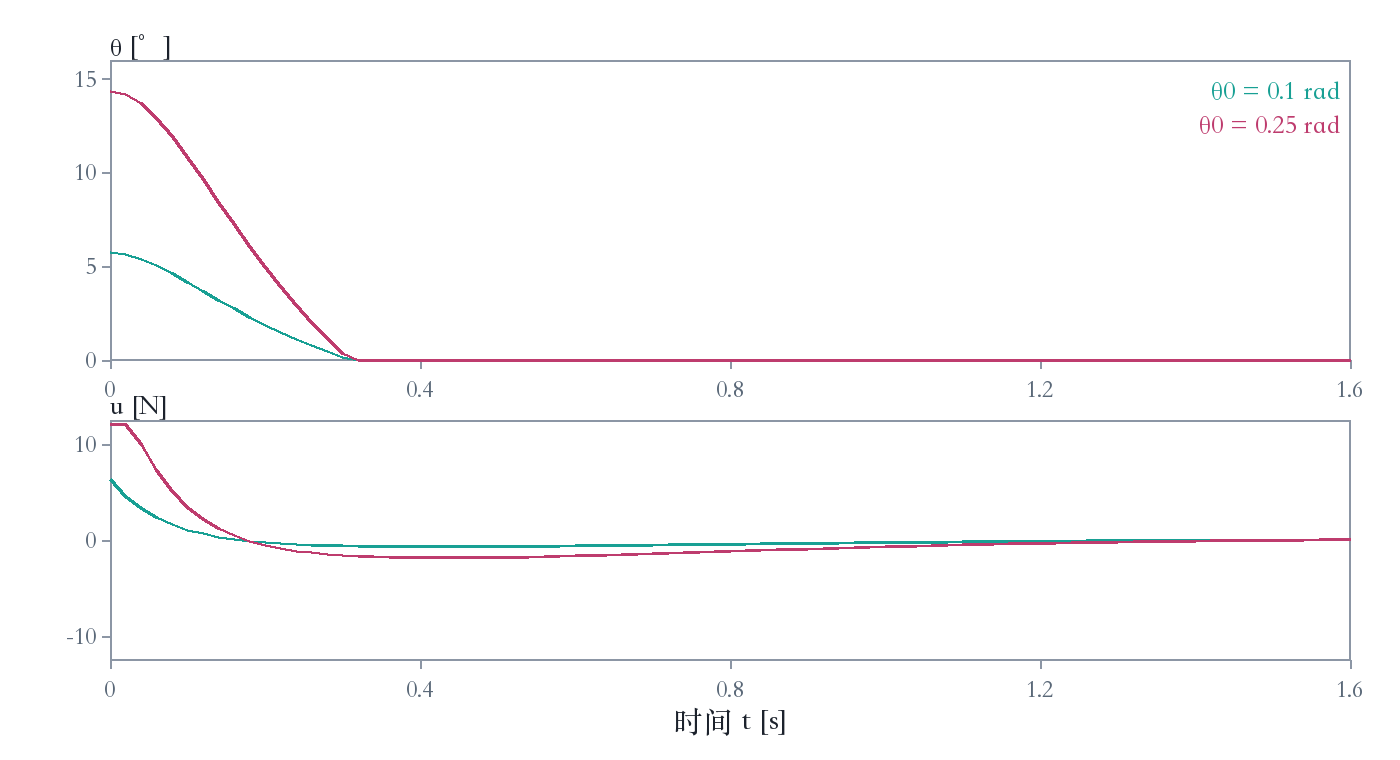
\includegraphics[width=0.92\linewidth]{figures/response.png}
\caption{两个初始角度下的闭环响应：上图为倾角 $\theta(t)$，下图为控制力 $u(t)$。
$0.1$\,rad 出发时峰值力只有 $6.3$\,N；$0.25$\,rad 时开始触及 $12$\,N 限幅，
之后收敛明显变慢（$0.24$\,s $\to$ $1.36$\,s）。\textbf{执行器饱和是第一个真正的非线性}。}
\label{fig:response}
\end{figure}

这里有一个容易被忽略的细节：$0.1$\,rad 到 $0.25$\,rad，初值只大了 $2.5$ 倍，
收敛时间却从 $0.24$\,s 涨到 $1.36$\,s——\textbf{涨了 5.7 倍}。
原因不是"LQR 变差了"，而是力被限幅截断，线性最优解在饱和之后就失效了。
线性控制理论的一切结论都建立在"$u$ 不受限"上。

\section{吸引域：把"局部"画出来}

\subsection{定义与算法}

\begin{quote}
\textbf{吸引域}（region of attraction）：所有能让闭环系统收敛到直立平衡点的初值集合。
\end{quote}

三维状态没法直接画，于是固定 $p_0=\dot p_0=0$，在 $(\theta_0,\dot\theta_0)$ 平面上扫描：

\begin{enumerate}[leftmargin=2em,itemsep=2pt]
  \item 网格：$\theta_0\in[-1.2,1.2]$（61 点）$\times$ $\dot\theta_0\in[-4,4]$（81 点）；
  \item 每个点跑 $3$\,s 闭环仿真；
  \item 判据：过程不撞墙，且末端 $|\theta|<0.05$\,rad、$|p|<1.5$\,m。
\end{enumerate}

共 $61\times81=4941$ 次仿真，结果见图 \ref{fig:basin}。

\begin{figure}[htbp]
\centering
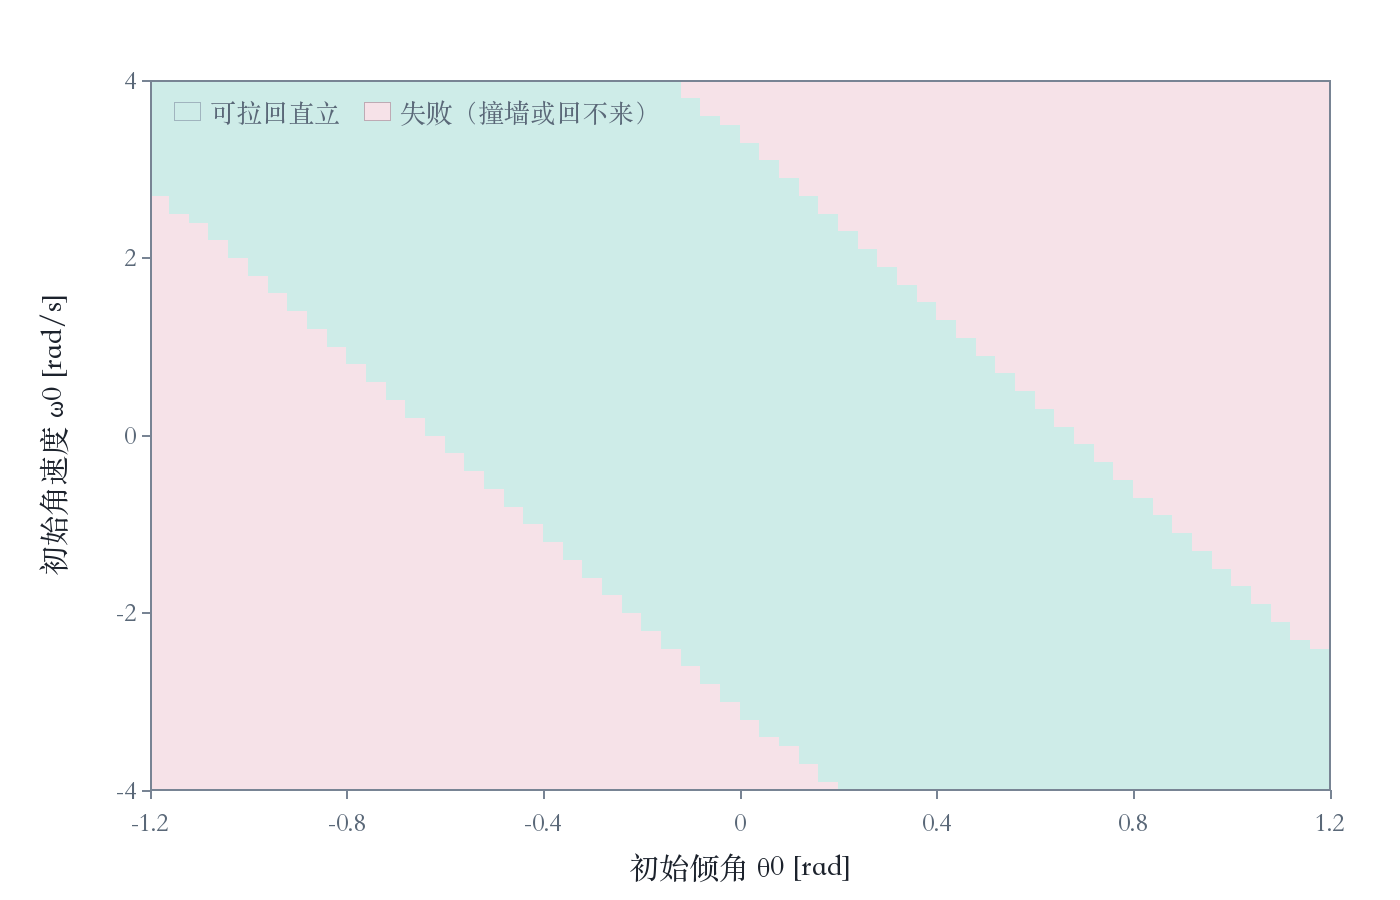
\includegraphics[width=0.86\linewidth]{figures/basin.png}
\caption{LQR 的吸引域。浅色区域能从该初值拉回直立，深色区域失败。
边界不是圆，而是一条\textbf{斜带}：同样大的倾角，如果摆正在朝直立方向转
（$\theta_0>0,\dot\theta_0<0$），容错就大得多。整体关于原点严格点对称
（$4941$ 个格子中 $0$ 个不对称），这来自被控对象的对称性。}
\label{fig:basin}
\end{figure}

\subsection{读图}

\begin{itemize}[leftmargin=2em,itemsep=3pt]
  \item \textbf{面积}：成功区域占整个扫描矩形的 $51.8\%$。
  \item \textbf{静止释放的极限}：$\dot\theta_0=0$ 时，能救回的最大倾角是 $\theta_{\max}=0.64$\,rad
        （约 $37^\circ$）。超过这个角度，无论怎么推都来不及。
  \item \textbf{斜带}：在 $\dot\theta_0=-4$\,rad/s（快速朝直立方向转）时，$\theta_0$ 可以大到 $1.2$\,rad；
        反过来，如果摆正在\textbf{远离}直立的方向快速旋转，能救的范围就小得多。
  \item \textbf{点对称}：把图旋转 $180^\circ$ 与自身完全重合。这说明边界是被控对象的性质，
        不是控制器或仿真器的缺陷。
\end{itemize}

\section{全局失败：$25\%$ 与 $82\%$}

把同一份参数丢到"真实任务"里：$60$ 组随机初值（$\theta_0$ 在整圈上均匀分布、$p_0\in\pm1$\,m），
$12$\,s 闭环，成功判据同第 1 讲。

\begin{center}
\small
\begin{tabular}{@{}lcc@{}}
\toprule
指标 & LQR（本讲） & 说明 \\
\midrule
成功率 & $25\%$ & 只有四分之一的初值能被救回来 \\
撞墙率 & $82\%$ & 绝大多数回合把车推到导轨尽头 \\
末端 $|\theta|$ 均值 & $1.62$\,rad & 失败回合基本是"躺平"或"乱转" \\
平均 $|p|_{\max}$ & $2.17$\,m & 几乎贴着 $2.4$\,m 的导轨极限 \\
\bottomrule
\end{tabular}
\end{center}

\subsection{失败是怎么发生的}

从下垂位置（$\theta_0=\pi-0.1$）出发，LQR 的行为可以逐秒复述：

\begin{enumerate}[leftmargin=2em,itemsep=2pt]
  \item $0$--$0.3$\,s：$\theta\approx\pi$，$K_\theta\theta\approx-191$\,N 远超限幅，
        于是 $u=+12$\,N 立刻饱和（推力朝右，因为在本讲约定里 $\theta>0$ 表示"摆向右倾"）；
  \item $0.3$--$1.5$\,s：车被推向右侧极限，摆杆因为小车加速而略有摆动，
        但幅度远不足以翻上来；
  \item 之后：车撞墙（位置钳位、速度清零），摆继续倒下或乱转，控制量来回打满。
\end{enumerate}

\keypoint{LQR 的失败不是因为"参数没调好"，而是因为它在 $\theta\approx\pi$ 处的
\textbf{线性化模型完全错了}：第 1 讲已经量化过，$1$\,s 后线性化预测与实际相差 $35\%$，
更何况 $\pm\pi$ 附近 $\sin\theta\approx\theta$ 的假设早已失效。
换句话说——\textbf{它在用一个错误的地图全力导航}。}

\subsection{一个反直觉的现象}

当 $\theta$ 接近 $\pi$ 时，$K_\theta\cdot\theta$ 这一项会给出巨大的力
（$62.89\times3.14\approx197$\,N，远超 $12$\,N 限幅），所以控制器\textbf{永远处于饱和}。
饱和之后，闭环就退化成"恒定 $-12$\,N 的开环推力"，摆当然不会立起来。
这解释了一个常见误解：\emph{以为换个更好的 $Q,R$ 就能全局收敛}。
实际上表 \ref{tab:designs} 会看到，增大增益只会让饱和更早发生，吸引域几乎不变。

\section{$Q/R$ 怎么选：三组设计的对比}

\begin{center}
\small
\begin{tabular}{@{}lcccccc@{}}
\toprule
设计 & $Q$ & $R$ & $K_\theta$ & 收敛时间 & 峰值力 & 吸引域占比 \\
\midrule
温和 & $\mathrm{diag}(1,10,0.3,0.5)$ & $1.0$ & $-27.5$ & $1.96$\,s & $12$\,N & $37\%$ \\
默认 & $\mathrm{diag}(1,40,1,2)$ & $0.05$ & $-62.9$ & $1.36$\,s & $12$\,N & $52\%$ \\
激进 & $\mathrm{diag}(1,120,3,5)$ & $0.01$ & $-178.5$ & $1.36$\,s & $12$\,N & $52\%$ \\
\bottomrule
\end{tabular}
\captionof{table}{三组 $Q/R$ 的对比（$\theta_0=0.25$\,rad 出发）。}
\label{tab:designs}
\end{center}

读这张表有两个结论：

\begin{enumerate}[leftmargin=2em,itemsep=2pt]
  \item \textbf{$Q/R$ 决定"多激进"，不决定"能走多远"}。温和→默认，收敛时间从 $1.96$\,s
        降到 $1.36$\,s，吸引域从 $37\%$ 涨到 $52\%$；但默认→激进，两个指标\textbf{都不再改善}。
  \item \textbf{天花板是执行器}。激进设计把 $K_\theta$ 从 $63$ 提到 $179$，但峰值力早就顶到 $12$\,N，
        更高的增益只是让饱和更早、更久。\textbf{在饱和世界里，增益不是免费的。}
\end{enumerate}

\keypoint{这一节给出了本讲的中心结论：\textbf{局部最优 ≠ 全局可行}。
在一个 $25\%$ 成功率的世界里，把一个 $0.64$\,rad 的吸引域再优化 $20\%$ 没有意义；
真正缺的是"从头到尾"的策略——那就需要第 4 讲的能量、第 6 讲的切换。}

\section{从失败读出设计需求}

把上面的观察翻译成三条设计需求，正好对应后面三讲：

\begin{center}
\small
\begin{tabular}{@{}lp{4.4cm}p{4.4cm}@{}}
\toprule
观察 & 需求 & 对应讲 \\
\midrule
$\theta$ 大时线性模型失效 & 需要一个不依赖小角假设的全局控制律 & 第 4 讲（能量整定）\\
饱和让"更强的反馈"失效 & 需要主动管理能量而不是被动加增益 & 第 4、5 讲 \\
没有位置积分、抗扰差 & 需要把鲁棒性写进结构 & 第 5 讲（滑模）\\
两个目标（位置/角度）争一个输入 & 需要按状态分区、显式切换 & 第 6 讲（监督器）\\
\bottomrule
\end{tabular}
\end{center}

\section{本讲小结}

\begin{enumerate}[leftmargin=2em,itemsep=2pt]
  \item LQR 通过解 CARE 得到最优线性反馈：$K=[-4.47,-62.89,-9.31,-16.40]$，
        闭环极点 $\{-11.96,-4.43,-0.90\pm0.47j\}$，阻尼比 $0.89$。
  \item 局部表现极好：$0.1$\,rad 出发 $0.24$\,s 进入 $\pm0.02$\,rad，峰值力只有 $6.3$\,N。
  \item 吸引域是一条\textbf{斜带}：静止释放的极限倾角 $0.64$\,rad，面积占比 $51.8\%$，
        关于原点严格点对称。
  \item 全局失败：$25\%$ 成功率、$82\%$ 撞墙率。失败根源是\textbf{线性化在地图之外失效}
        加上\textbf{力被限幅}，而不是参数没调好。
  \item $Q/R$ 只能调"多激进"，调不动"能走多远"；天花板由执行器决定。
\end{enumerate}

\section*{习题}
\addcontentsline{toc}{section}{习题}

\begin{enumerate}[leftmargin=2em,itemsep=6pt]
  \item 手算验证 $K_\theta/K_p\approx 14$ 的由来：从 CARE 出发，解释为什么重罚 $\theta$
        会让这两个分量的比例变大。
  \item 把 $R$ 从 $0.05$ 调到 $0.5$，重算 $K$ 与闭环极点，并解释阻尼比的变化方向。
  \item 只用 $p,\theta$ 两个状态（去掉速度反馈，即 $K_{\dot p}=K_{\dot\theta}=0$）
        重新设计，看吸引域缩小多少，并解释原因。
  \item 让 $u_{\max}$ 从 $12$\,N 增加到 $20$\,N，重跑吸引域扫描：面积占比变成多少？
        这说明"能力边界"主要由什么决定？
  \item 在 $\theta_0=0.6$\,rad、$\dot\theta_0=0$ 的边界附近，画出 $\theta(t)$ 的相图，
        观察它是"刚好回来"还是"擦边失败"。
  \item （编程）复现 \S2.4 的吸引域扫描，并把判据从"$3$\,s 内收敛"改成"$6$\,s 内收敛"，
        看边界变化多少。这个敏感性说明了什么？
\end{enumerate}

\section*{延伸阅读}
\addcontentsline{toc}{section}{延伸阅读}
\begin{itemize}[leftmargin=2em,itemsep=2pt]
  \item B. D. O. Anderson, J. B. Moore, \emph{Optimal Control: Linear Quadratic Methods},
        Dover, 2007.（CARE 的完整推导与数值解法）
  \item R. Tedrake, \emph{Underactuated Robotics}, 第 8 章：LQR 与轨迹优化。
  \item 关于吸引域的计算：E. Najafi et al., \emph{Computing the region of attraction...},
        CDC 2016（平方和规划与网格法的对比）。
\end{itemize}

\chapter[反馈线性化]{第 3 讲\quad 部分反馈线性化：把"力"变成"加速度"}
\label{ch:fbl}

\begin{quote}\small
\textbf{本讲目标}\quad 换一个坐标看同一台机器：把"我能施加多大力"换成"我能让小车产生多大加速度"。
小车通道是完全驱动的，所以这个换元是\textbf{精确}的、全域可逆的。换完之后，
后面所有控制器都只需要对付摆杆那一个非线性方程。\\[2pt]
\textbf{前置}\quad 第 1 讲的状态方程；第 2 讲的"局部最优"概念。\\
\textbf{视频}\quad 约 3 分钟。\quad\textbf{代码}\quad \texttt{build/controllers.py: cart\_inverse\_dynamics}。
\end{quote}

\section{为什么值得换坐标}

回顾第 1 讲的两个方程：
\begin{align}
  (m_c+m_p\sin^2\theta)\,\ddot p &= u - b_c\dot p + m_p l\sin\theta\,\dot\theta^2
     + b_p\cos\theta\,\dot\theta - m_p g\sin\theta\cos\theta,\\
  \ddot\theta &= \frac{g\sin\theta - \ddot p\cos\theta - b_p\dot\theta/(m_p l)}{l}.
\end{align}
对控制器设计者来说，这两个式子很讨厌：摩擦、科氏项、重力耦合全混在一起，
每设计一个控制律都要把这些项重新算一遍。

但如果把视角从"力 $u$"换成"小车加速度 $\ddot p$"，情况完全不同：
上式左端的分母恒正（第 1 讲命题 1），于是\textbf{对任意给定的 $\ddot p$，
都有一个唯一的力与之对应}。把这件事写成映射：

\begin{equation}
  u = \underbrace{\big(m_c+m_p\sin^2\theta\big)}_{\text{等效质量}}\,\ddot p
      + \underbrace{b_c\dot p - m_p l\sin\theta\,\dot\theta^2
        - b_p\cos\theta\,\dot\theta + m_p g\sin\theta\cos\theta}_{\text{需要抵消的"干扰"}} .
  \label{eq:inv}
\end{equation}

\keypoint{式 \eqref{eq:inv} 是\textbf{精确}的，不是近似。
它把系统拆成两层：内层负责"抵消已知的非线性"，外层面对一个干净的输入 $v=\ddot p$。
这就是\textbf{部分反馈线性化}（partial feedback linearization）——
"部分"是因为只线性化了小车通道，摆杆通道依旧是非线性的。}

\section{相对阶：为什么只挑小车通道}

对输出 $y=p$，求导两次就出现 $u$（因为 $\ddot p$ 显含 $u$），所以相对阶是 2。
对输出 $y=\theta$，有
\begin{equation}
  \ddot\theta = \frac{g\sin\theta - \ddot p\cos\theta}{l} - \frac{b_p\dot\theta}{m_p l^2},
\end{equation}
其中 $\ddot p$ 显含 $u$，但系数是 $\cos\theta$。因此\textbf{只要 $\cos\theta\ne0$，
$\theta$ 的相对阶也是 2}。

两个输出都是 2 阶，系统总阶是 4，输入只有 1 个。解耦矩阵
\begin{equation}
  \Delta(x) = \begin{bmatrix}
    \dfrac{1}{m_c+m_p\sin^2\theta}\\[8pt]
    \dfrac{-\cos\theta}{l\,(m_c+m_p\sin^2\theta)}
  \end{bmatrix}\in\mathbb{R}^{2\times1}
\end{equation}
是一个\textbf{列向量}，秩恒为 1。所以不可能同时把 $\ddot p$ 和 $\ddot\theta$ 指定成任意值——
这就是第 1 讲说过的欠驱动。工程上的处理是：\textbf{只线性化能线性化的那个通道，
把另一个通道交给"能量"或"滑模"去管}。

\section{反解之后系统长什么样}

把 \eqref{eq:inv} 代入原方程，得到
\begin{empheq}[box=\fbox]{align}
  \ddot p &= v \qquad(\text{单位增益，精确线性化})\\
  \ddot\theta &= \frac{g\sin\theta - v\cos\theta}{l}
     - \frac{b_p\dot\theta}{m_p l^2}
  \label{eq:after}
\end{empheq}
其中 $v$ 是新的控制输入（加速度指令）。

\begin{itemize}[leftmargin=2em,itemsep=2pt]
  \item \textbf{小车通道变成二重积分器}：$p^{(2)}=v$，这是控制理论里最好对付的对象。
  \item \textbf{摆杆通道保留全部非线性}，但形式变干净了：只剩 $g\sin\theta$ 和 $v\cos\theta$，
        以及一个很小的粘性项。后面第 4、5 讲都在这一个方程上做文章。
\end{itemize}

\section{精度验证}

反解是解析的，所以精度只受两个因素影响：浮点误差与\textbf{限幅}。
数值实验（$200$ 组随机状态与随机指令 $v$，用 $10^{-4}$\,s 步长估计实际 $\ddot p$）：

\begin{center}
\small
\begin{tabular}{@{}lcc@{}}
\toprule
指标 & 数值 & 说明 \\
\midrule
最大误差 $|\ddot p - v|$ & $9.2\times10^{-4}$\,m/s$^2$ & 出现在指令被 $\pm12$\,N 限幅的样本 \\
平均误差 & $2.2\times10^{-4}$\,m/s$^2$ & 相当于 $0.02\%$ 的相对误差 \\
\bottomrule
\end{tabular}
\end{center}

\begin{quote}
换句话说：\textbf{只要不加限幅，这个反解在数值上就是恒等式}。
真正让"精确线性化"失效的不是数学，而是执行器——这一点在后续每一讲都会反复出现。
\end{quote}

\section{奇异点：摆杆通道会失去权限}

式 \eqref{eq:after} 中 $\cos\theta$ 是 $v$ 的系数。当 $\theta\to\pm90^\circ$ 时：

\begin{center}
\small
\begin{tabular}{@{}ccc@{}}
\toprule
$\theta$ & $\cos\theta$ & 小车加速度对 $\ddot\theta$ 的影响 \\
\midrule
$0^\circ$ & $1.00$ & 满权限 \\
$30^\circ$ & $0.87$ & $87\%$ \\
$60^\circ$ & $0.50$ & 一半 \\
$80^\circ$ & $0.17$ & 几乎失效 \\
$90^\circ$ & $0$ & \textbf{完全失效} \\
\bottomrule
\end{tabular}
\end{center}

这个表解释了一件重要的事：\textbf{摆杆水平时，无论小车怎么加速，都改变不了它的角加速度}。
所以在第 5 讲的滑模控制器里，我们对 $\cos\theta$ 做了钳位（$|\cos\theta|\ge0.25$），
并在 $\theta$ 较大时根本不使用依赖 $1/\cos\theta$ 的通道——那段交给摆起控制器。

\section{"换坐标"到底带来多少好处}

一个直接对照实验：同样的能量整定律 $v = k_E(E-E_d)\,\mathrm{sat}(\dot\theta\cos\theta/\phi)$，

\begin{center}
\small
\begin{tabular}{@{}lccc@{}}
\toprule
实现方式 & 最佳 $k_E$ & 能把摆送到顶的比例 & 说明 \\
\midrule
直接调力（无力矩补偿） & $6.0$ & $0/3$ & 冷启动时摩擦与耦合项吃掉能量 \\
加速度域（式 \eqref{eq:inv}） & $6.0$ & $3/3$ & 同一增益下全部成功 \\
\bottomrule
\end{tabular}
\end{center}

同一个控制律、同一个增益，只因为中间加了一层精确反解，就从"一个都上不去"变成"全部上去"。
这不是玄学：能量泵的推导假设"$v$ 可以任意指定"，而直接调力时这个假设根本不成立。

\keypoint{这就是"反馈线性化"的实际价值：它不是为了炫技，
而是为了\textbf{让外环控制律的推导前提成立}。}

\section{本讲小结}

\begin{enumerate}[leftmargin=2em,itemsep=2pt]
  \item 小车通道完全驱动 $\Rightarrow$ 式 \eqref{eq:inv} 是精确反解，全域可逆。
  \item 反解后系统变成 $p^{(2)}=v$ 加一个仍非线性的摆杆方程 \eqref{eq:after}。
  \item 精度验证：不作限幅时反解误差 $\sim10^{-4}$，本质上是恒等式。
  \item 奇异点：$\cos\theta\to0$ 时摆杆通道失去权限，必须显式处理。
  \item 同一能量整定律，加了反解才能工作（$0/3\to3/3$）。
\end{enumerate}

\section*{习题}
\addcontentsline{toc}{section}{习题}
\begin{enumerate}[leftmargin=2em,itemsep=6pt]
  \item 从式 \eqref{eq:pdd_raw} 出发，独立推导 \eqref{eq:inv}，并验证各项符号。
  \item 若改为指定摆杆加速度（令 $\ddot\theta=w$），反解会多出一个什么奇异项？
        在什么角度附近数值上会爆炸？
  \item 在式 \eqref{eq:inv} 中逐项去掉"干扰"（摩擦、科氏、重力耦合），
        各做一次仿真，看能量泵的成功率下降多少。
  \item 把 $\cos\theta$ 的钳位从 $0.25$ 改成 $0.1$ 与 $0.5$，观察滑模控制器给不出指令的角度范围。
  \item （编程）用 $10^{-2}$ 到 $10^{-5}$ 的步长验证反解精度，画误差随步长的收敛曲线。
\end{enumerate}

\section*{延伸阅读}
\addcontentsline{toc}{section}{延伸阅读}
\begin{itemize}[leftmargin=2em,itemsep=2pt]
  \item J.-J. Slotine, W. Li, \emph{Applied Nonlinear Control}, 第 6 章（输入–输出线性化与零动态）。
  \item S. Fantoni, R. Lozano, \emph{Non-linear Control for Underactuated Mechanical Systems}, 第 2 章。
\end{itemize}

\chapter[能量整定]{第 4 讲\quad 能量整定：把"摆起来"变成标量目标}
\label{ch:energy}

\begin{quote}\small
\textbf{本讲目标}\quad 用一个标量（能量）代替"姿态轨迹"，让摆从下垂自己甩到竖直附近。
给出控制律、Lyapunov 证明、以及一个真实的工程坑：小车会跑。\\[2pt]
\textbf{前置}\quad 第 3 讲的加速度域 $p^{(2)}=v$。\\
\textbf{视频}\quad 约 3 分钟。\quad\textbf{代码}\quad \texttt{controllers.py: EnergyFBL}。
\end{quote}

\section{能量通道}

在第 3 讲的加速度域里，摆杆方程是
\begin{equation}
  \ddot\theta=\frac{g\sin\theta-v\cos\theta}{l}-\frac{b_p\dot\theta}{m_p l^2}.
\end{equation}
定义摆杆相对直立静止的能量
\begin{equation}
  E=\tfrac12 m_p l^2\dot\theta^2+m_p g l(\cos\theta-1),
  \label{eq:E}
\end{equation}
求导并代入上式，得到这一讲最重要的一个式子：
\begin{equation}
  \boxed{\;\dot E=-m_p l\,(\dot\theta\cos\theta)\,v-b_p\dot\theta^2\;}
  \label{eq:dE}
\end{equation}

\begin{quote}
\textbf{读法}：$v$ 与 $\dot\theta\cos\theta$ 是一对"功"的共轭量。
只要让加速度与 $\dot\theta\cos\theta$ 同号，能量就上升；反号就下降。
\textbf{控制能量，就是控制这一对量的相位。}
\end{quote}

\section{控制律与 Lyapunov 证明}

取
\begin{equation}
  v=k_E\,(E-E_d)\,\mathrm{sat}\!\left(\frac{\dot\theta\cos\theta}{\phi}\right)
   -k_x p-k_d\dot p,\qquad E_d=0 .
  \label{eq:law}
\end{equation}
忽略阻尼项与回中项，代入 \eqref{eq:dE}：
\begin{align}
  \dot E &= -m_p l\,k_E (E-E_d)\,(\dot\theta\cos\theta)\,
            \mathrm{sat}\!\left(\frac{\dot\theta\cos\theta}{\phi}\right)\\
         &= -m_p l\,k_E (E-E_d)\,\big|\dot\theta\cos\theta\big|\,
            \Big|\mathrm{sat}(\cdot)\Big| \;\le 0 \quad(\text{当 } E>E_d).
\end{align}
取 $W=\tfrac12(E-E_d)^2$，则
\begin{equation}
  \dot W=(E-E_d)\dot E
  =-m_p l\,k_E\,(E-E_d)^2\,\big|\dot\theta\cos\theta\big|\,\big|\mathrm{sat}(\cdot)\big|\le0 .
\end{equation}

\begin{quote}
$W$ 单调不增，故 $E\to E_d$。收敛速度正比于 $|\dot\theta\cos\theta|$——
\textbf{摆不动的时候泵不进能量}，这既是物理事实，也是后面的坑。
\end{quote}

\section{LaSalle 与"下垂陷阱"}

用 LaSalle 不变集原理：$\dot W=0$ 要求 $|\dot\theta\cos\theta|=0$，即
$\dot\theta=0$ 或 $|\cos\theta|=0$。能长期停留的不变集有两个：

\begin{enumerate}[leftmargin=2em,itemsep=2pt]
  \item $\theta=0,\ \dot\theta=0$：\textbf{直立静止}，$E=0=E_d$ ✓ 目标；
  \item $\theta=\pi,\ \dot\theta=0$：\textbf{下垂静止}，$E=-2m_pgl\ne E_d$ ✗ 陷阱。
\end{enumerate}

第二个是\\textbf{测度为零的对称点}：真实系统任何微小扰动都会打破它。
工程上的处理是让"下垂"这个初值永远带上一点偏差（本课用 $\theta_0=\pi-0.14$），
或者加一个极小的抖动项（dither）。

\section{为什么必须加"小车回中"}

式 \eqref{eq:law} 的前半段只关心能量，完全不关心小车在哪。仿真里会发生两件事：

\begin{enumerate}[leftmargin=2em,itemsep=2pt]
  \item 泵能量需要小车持续加速，于是\textbf{小车被越推越远}；
  \item 一旦撞墙（位置钳位、速度清零），能量泵就断了——摆还没到顶就失去动力。
\end{enumerate}

所以必须加 $-k_xp-k_d\dot p$。但这两个系数不能大：\textbf{回中本身在消耗能量}。
表 \ref{tab:kx} 是本课的实测（固定 $k_E=6$，三个初值）：

\begin{center}
\small
\begin{tabular}{@{}ccc@{}}
\toprule
$k_x/k_d$ & 平均摆起时间 & 平均 $|p|_{\max}$ \\
\midrule
$0.35\,/\,0.45$ & 未抓到（$>15$\,s） & $1.42$\,m \\
$0.90\,/\,1.30$ & $3.6$\,s & $1.85$\,m \\
$1.30\,/\,1.90$ & $3.1$\,s & $2.37$\,m \\
\bottomrule
\end{tabular}
\captionof{table}{回中增益的权衡：太弱赶不上，太强撞墙。}
\label{tab:kx}
\end{center}

\section{增益 $k_E$：泵多快，撞多狠}

$k_E$ 决定"一次摆动能泵入多少能量"，是本讲最关键的参数。实测（三个初值平均）：

\begin{center}
\small
\begin{tabular}{@{}cccc@{}}
\toprule
$k_E$ & 平均摆起时间 & 平均 $|p|_{\max}$ & 结果 \\
\midrule
$1.0$ & $>15$\,s & $0.81$\,m & 泵得太慢，15\,s 内抓不住 \\
$2.0$ & $>15$\,s & $1.25$\,m & 同上 \\
$3.0$ & $>15$\,s & $1.62$\,m & 同上 \\
$4.0$ & $>15$\,s & $1.94$\,m & 同上 \\
$6.0$ & $3.13$\,s & $2.37$\,m & 可用（接近导轨极限） \\
$8.0$ & $2.35$\,s & $2.60$\,m & 撞墙（超过 $2.4$\,m） \\
\bottomrule
\end{tabular}
\end{center}

这条曲线不是单调的"越大越好"：\textbf{泵得越猛，摆起越快，但小车走得越远}。
$k_E=6$ 是"刚好能在导轨内完成一次摆起"的临界点附近——这也是本课最终选它的原因。

\section{实测：一次完整的摆起}

从 $\theta_0=\pi-0.14$ 出发，闭环 $12$\,s 的关键数字：

\begin{center}
\small
\begin{tabular}{@{}lc@{}}
\toprule
指标 & 数值 \\
\midrule
能量初值 & $-2.93$\,J（下垂）\\
能量峰值 & $+0.026$\,J（略有过冲，随后被 LQR 拉回 0）\\
首次进入 $|\theta|<0.1$\,rad & $1.98$\,s \\
$|p|_{\max}$ & $2.37$\,m（离导轨极限还有 3\,cm）\\
稳态 $|\theta|$ & $<10^{-3}$\,rad \\
\bottomrule
\end{tabular}
\end{center}

\begin{quote}
注意"能量峰值 $+0.026$"这个细节：能量控制\textbf{不会精确停在 0}，
它会把摆"抛过头"一点点，然后由第 6 讲的切换器接管。这正是"摆起"和"稳摆"必须分开的原因。
\end{quote}

\section{本讲小结}
\begin{enumerate}[leftmargin=2em,itemsep=2pt]
  \item 能量导数 $\dot E=-m_p l(\dot\theta\cos\theta)v-b_p\dot\theta^2$ 把控制问题变成"相位"问题。
  \item $W=\tfrac12(E-E_d)^2$ 是合法 Lyapunov 函数，$W$ 单调不增。
  \item LaSalle 给出两个不变集：直立的（目标）与下垂的（陷阱）。
  \item 回中项必须"慢"，$k_E$ 必须"刚好"：$k_E$ 太小抓不住，太大撞墙。
  \item 摆起完成时能量会略微过冲，需要局部稳定器接管 —— 引出第 5、6 讲。
\end{enumerate}

\section*{习题}
\addcontentsline{toc}{section}{习题}
\begin{enumerate}[leftmargin=2em,itemsep=6pt]
  \item 从 \eqref{eq:E} 出发独立推导 \eqref{eq:dE}，说明 $-b_p\dot\theta^2$ 项的来源。
  \item 若去掉 $\mathrm{sat}(\cdot)$ 直接用 $\mathrm{sign}(\cdot)$，会发生什么？用仿真验证抖振。
  \item 证明：当 $E<E_d$ 时 \eqref{eq:law} 的第一个因子为负，因此 $v$ 与 $\dot\theta\cos\theta$ 反号。
  \item 把 $\phi$ 从 $0.05$ 调到 $1.0$，观察摆起时间与力的平滑度如何变化。
  \item 设计一个"自适应 $k_E$"：当 $|p|>1.8$\,m 时降低泵增益，看能否避免撞墙。
  \item （编程）复现表 4.2 的 $k_E$ 扫描，并画出"摆起时间–撞墙率"的帕累托前沿。
\end{enumerate}

\section*{延伸阅读}
\addcontentsline{toc}{section}{延伸阅读}
\begin{itemize}[leftmargin=2em,itemsep=2pt]
  \item K. J. Åström, K. Furuta, \emph{Swinging up a pendulum by energy control}, Automatica 36(2), 2000.
  \item M. W. Spong, \emph{Energy based control of a class of underactuated mechanical systems}, IFAC 1996.
\end{itemize}

\chapter[滑模]{第 5 讲\quad 滑模控制：把鲁棒性做进结构}
\label{ch:smc}

\begin{quote}\small
\textbf{本讲目标}\quad 上一讲的局部稳定器是 LQR——它完全相信模型。本讲换一种思路：
先规定一条"必须到达的流形"，再用力把状态按死在流形上。代价是抖振，收益是抗扰。\\[2pt]
\textbf{前置}\quad 第 3 讲的加速度域；第 4 讲的"局部稳定器替换"。\\
\textbf{视频}\quad 约 3 分钟。\quad\textbf{代码}\quad \texttt{controllers.py: SMC}。
\end{quote}

\section{从"相信模型"到"规定流形"}

LQR 的隐含假设是：$A,B$ 准确、无外部扰动。实际系统里这两条都不成立
（第 2 讲已经看到：$4$\,N 侧风就能让稳态角度偏 $0.014$\,rad）。

滑模控制换一个问法：

\begin{quote}
\textbf{与其问"最优反馈是什么"，不如问"我希望状态被约束在哪个低维集合上"。}
\end{quote}

对摆杆，我们希望 $\theta$ 以某个速率衰减到 0，于是取
\begin{equation}
  s=\dot\theta+\lambda(\theta-\theta_{\mathrm{ref}}),\qquad \lambda>0 .
  \label{eq:surface}
\end{equation}
$s=0$ 是相平面上一条直线：\textbf{只要保持在上面，$\theta$ 就按 $e^{-\lambda t}$ 衰减}。
这把"二维跟踪问题"降成了"一维镇定问题"。

\section{到达律}

规定 $s$ 的收敛方式（到达律）：
\begin{equation}
  \dot s=-\eta\,\mathrm{sat}(s/\phi)-k_s s,\qquad \eta>0,\ \phi>0 .
  \label{eq:reach}
\end{equation}
其中 $\mathrm{sat}(\cdot)$ 是带边界层的符号函数：
\begin{equation}
  \mathrm{sat}(x)=\begin{cases}
    x, & |x|\le1,\\
    \mathrm{sign}(x), & |x|>1 .
  \end{cases}
\end{equation}

\begin{itemize}[leftmargin=2em,itemsep=2pt]
  \item $\eta$ 是\textbf{抗扰强度}：$|扰动|<\eta$ 时，扰动无法把 $s$ 推出边界层。
  \item $\phi$ 是\textbf{边界层宽度}：$|s|<\phi$ 时用线性反馈（无抖振），
        $|s|>\phi$ 时用等效符号函数（强鲁棒）。$\phi\to0$ 就是经典滑模，代价是抖振。
  \item $k_s$ 是普通的比例项，加速进入边界层。
\end{itemize}

\section{解出加速度指令}

把 $\ddot\theta=(g\sin\theta-v\cos\theta)/l-b_p\dot\theta/(m_pl^2)$ 代入 $\dot s$，解出 $v$：
\begin{equation}
  v=\frac{g\sin\theta+l\big[\lambda\dot\theta+\eta\,\mathrm{sat}(s/\phi)+k_s s\big]}{\cos\theta}.
  \label{eq:vsmc}
\end{equation}

这个式子有两个必须处理的工程细节：

\begin{enumerate}[leftmargin=2em,itemsep=2pt]
  \item \textbf{$1/\cos\theta$ 奇异}：第 3 讲已经量化过，$\theta\to\pm90^\circ$ 时它发散。
        实现里把 $|\cos\theta|$ 钳位到 $\ge0.25$（对应 $\theta\le75.5^\circ$）。
  \item \textbf{单输入两个目标}：式 \eqref{eq:vsmc} 只负责 $\theta$，小车位置没人管。
        详见 \S5.5。
\end{enumerate}

\section{边界层与抖振}

$\phi$ 越小，鲁棒性越强、抖振越大。极限情况 $\phi\to0$ 时，控制量在
$v=\pm\infty$ 之间以开关频率跳变——真实执行器会被打坏。

工程折中：$\phi$ 取"传感器噪声量级 + 执行器带宽允许的切换频率"。
本课参数 $\phi=0.25$（单位是 $s$ 的物理量纲 rad/s），在这个值下：
力矩的高频抖动 RMS 约 $0.02$\,N，对 $12$\,N 的执行器可以忽略。

\section{一个真实的坑：小车会跑}

式 \eqref{eq:vsmc} 不含 $p,\dot p$，所以小车会慢慢被推走。常见的错误做法是
"把 $-k_xp-k_d\dot p$ 直接加到 $v$ 上"：

\begin{quote}
\textbf{实测会发散}。原因是两个回路抢同一个输入：摆杆回路要求 $v$ 朝一个方向把 $s$ 压到 0，
回中回路却要求 $v$ 反向，两者叠加后 $s$ 被推出边界层，摆杆回路随即加大力度，形成极限环。
\end{quote}

正确的做法是\textbf{时间尺度分离}：让快速的摆杆回路去追踪一个极小的倾角偏置
\begin{equation}
  \theta_{\mathrm{ref}}=-\mathrm{clip}(k_pp+k_d\dot p,\ \pm0.25\ \mathrm{rad}).
  \label{eq:lean}
\end{equation}
当 $p>0$ 时 $\theta_{\mathrm{ref}}<0$，摆杆回路会把摆"摆向左侧"，于是小车被慢慢拉回原点。
摆杆回路依旧是主角，回中只是一个缓慢的参考漂移。

\keypoint{这条"倾斜参考"的技巧在多输入系统里叫\textbf{级联/时标分离}；
在单输入欠驱动系统里，它是唯一不引起回路冲突的回中方式。}

\section{抗扰实测}

统一协议：$40$ 组随机初值，第 4--8\,s 施加 $+4$\,N 侧向风，$12$\,s 闭环。

\begin{center}
\small
\begin{tabular}{@{}lccc@{}}
\toprule
局部稳定器 & 稳态 $|\theta|$ 均值 & 稳态 $|\theta|$ 峰值 & 力 RMS \\
\midrule
LQR（第 2 讲） & $0.0121$\,rad & $0.0412$\,rad & $2.46$\,N \\
SMC（本讲） & $\mathbf{0.0053}$\,rad & $0.0606$\,rad & $2.63$\,N \\
\bottomrule
\end{tabular}
\end{center}

读法：

\begin{itemize}[leftmargin=2em,itemsep=2pt]
  \item \textbf{平均误差降低 $2.3$ 倍}（$0.0121\to0.0053$）：到达律的 $\eta$ 项在持续风的条件下
        持续提供补偿，而 LQR 没有任何积分/鲁棒项。
  \item \textbf{峰值反而略大}（$0.0412\to0.0606$）：风刚加上去的瞬间，滑模还在"进入边界层"的过程中，
        有短暂的超调。这不影响长期精度，但提醒我们：\textbf{鲁棒性不是无延迟的}。
  \item \textbf{力 RMS 高 $7\%$}：鲁棒性是用控制能量换来的。
\end{itemize}

\section{本讲小结}
\begin{enumerate}[leftmargin=2em,itemsep=2pt]
  \item 滑模把跟踪问题降成一维镇定：$s=\dot\theta+\lambda(\theta-\theta_{\mathrm{ref}})$。
  \item 到达律 $\dot s=-\eta\,\mathrm{sat}(s/\phi)-k_s s$ 用 $\eta$ 换鲁棒、用 $\phi$ 换平滑。
  \item $1/\cos\theta$ 必须钳位，否则奇异。
  \item 小车回中必须走"倾斜参考"，直接叠加会与摆杆回路抢输入。
  \item 抗扰：稳态误差降 $2.3$ 倍，代价是力 RMS $+7\%$、瞬时峰值略大。
\end{enumerate}

\section*{习题}
\addcontentsline{toc}{section}{习题}
\begin{enumerate}[leftmargin=2em,itemsep=6pt]
  \item 从 $s$ 的定义出发，推导 $s$ 在 $s>0$ 与 $s<0$ 两侧的收敛速度，说明 $\eta/\phi$ 的作用。
  \item 计算 $\lambda=6$、$\phi=0.25$ 时，边界层对应多宽的 $\theta$ 区间（取 $\dot\theta=0$）。
  \item 把 $\eta$ 从 $6$ 调到 $30$，测力 RMS 与稳态误差，画出帕累托曲线。
  \item 若把钳位从 $0.25$ 改成不钳位，会发生什么？用 $\theta=85^\circ$ 附近的初值实验。
  \item （编程）复现表 5.1，并解释为什么 SMC 的峰值误差更大。
\end{enumerate}

\section*{延伸阅读}
\addcontentsline{toc}{section}{延伸阅读}
\begin{itemize}[leftmargin=2em,itemsep=2pt]
  \item V. Utkin, \emph{Sliding Modes in Control and Optimization}, Springer, 1992.
  \item J.-J. Slotine, S. S. Sastry, \emph{Tracking control of non-linear systems using sliding surfaces},
        Int. J. Control, 1983.
\end{itemize}

\chapter[切换与监督]{第 6 讲\quad 切换与监督：把两种局部真理缝起来}
\label{ch:switch}

\begin{quote}\small
\textbf{本讲目标}\quad 第 4 讲会甩、不会停；第 5 讲会停、不会甩。本讲把两者缝成一个控制器，
并讲清楚缝合处的三个工程问题：捕获窗口、迟滞带宽、切换瞬态。\\[2pt]
\textbf{前置}\quad 第 4 讲（能量）、第 5 讲（滑模或 LQR）。\\
\textbf{视频}\quad 约 2.5 分钟。\quad\textbf{代码}\quad \texttt{controllers.py: Hybrid}。
\end{quote}

\section{两种"局部真理"}

\begin{center}
\small
\begin{tabular}{@{}lll@{}}
\toprule
 & 能量整定（第 4 讲） & 局部稳定器（第 2/5 讲）\\
\midrule
擅长 & 大偏差：从任意角度把摆甩到顶上 & 小偏差：把误差压到 $10^{-3}$\,rad \\
不擅长 & 到顶后停不住（能量会过冲） & 角度一大模型就失效（吸引域外）\\
目标 & 把 $E$ 推到 $0$ & 把 $x$ 压到 $0$ \\
\bottomrule
\end{tabular}
\end{center}

两者互补，但\textbf{没有任何一个连续的反馈律能同时做到}（因为目标函数不同）。
所以必须\textbf{显式切换}。

\section{捕获窗口：多大才接得住}

切换的第一件事是定义"什么时候交给稳定器"。直觉是"$\theta$ 足够小的时候"，
但"足够小"到底是多少？实测（4 组初值，$15$\,s 闭环）：

\begin{center}
\small
\begin{tabular}{@{}cccc@{}}
\toprule
捕获阈值 $\theta_{\mathrm{in}}$ & 成功回合 & 说明 \\
\midrule
$0.25$\,rad & $0/4$ & 太窄：能量控制把摆"抛过"了竖直位置，接不住 \\
$0.35$\,rad & $4/4$ & 刚好 \\
$0.45$\,rad & $4/4$ & 更宽松，但仍然稳定 \\
$0.60$\,rad & $4/4$ & 接近 LQR 吸引域边界（$0.64$\,rad） \\
\bottomrule
\end{tabular}
\end{center}

\begin{quote}
\textbf{$0.25$\,rad 会全军覆没}，这件事很反直觉：窗口越窄，看起来越"安全"，实际越糟。
原因是能量控制到达顶点附近时，摆的速度不为零，$|\theta|<0.25$ 的时间窗可能只有几十毫秒——
而第 4 讲说过，切换是\textbf{在采样的瞬间发生的}，采样周期 $20$\,ms，
窗口太窄就会"看漏"。
\end{quote}

本课取 $\theta_{\mathrm{in}}=0.40$\,rad、$|\dot\theta|_{\mathrm{in}}=2.5$\,rad/s。

\section{迟滞：防止在边界上抖}

如果进入和退出用同一组阈值，噪声会让模式在临界点附近高频切换。做法是
\textbf{进出用不同阈值}：

\begin{center}
\small
\begin{tabular}{@{}lcc@{}}
\toprule
 & 进入稳摆 & 退回摆起 \\
\midrule
$|\theta|$ & $<0.40$ & $>0.80$ \\
$|\dot\theta|$ & $<2.5$ & $>3.5$ \\
\bottomrule
\end{tabular}
\end{center}

这两个区间之间的"死区"就是迟滞带。带宽太窄→抖振；太宽→摆已经掉下去了还在用 LQR。

\section{切换瞬态：$11$\,N 的单步跳变}

\begin{center}
\small
\begin{tabular}{@{}lccc@{}}
\toprule
控制器 & 切换次数 & 最大单步 $\Delta u$ & 首次到顶 \\
\midrule
能量 + LQR & $1$ & $11.0$\,N & $1.98$\,s \\
能量 + SMC & $1$ & $10.9$\,N & $1.90$\,s \\
\bottomrule
\end{tabular}
\end{center}

$11$\,N 的跳变意味着：切换那一帧，执行器的指令几乎从满幅正转到满幅负。
对真实电机，这是一次电流冲击；对仿真，它只是"不好看"。
\textbf{第 10 讲会看到，模仿学习学到的策略把这一跳变压到了 $5.4$\,N}——
这是数据驱动方法在本项目里唯一明确的优势。

\section{监督器设计清单}

把上面的经验固化成一张检查表，任何"多模式控制器"都适用：

\begin{enumerate}[leftmargin=2em,itemsep=3pt]
  \item \textbf{进入条件必须能被采样到}：切换窗口的时间宽度 $\gg$ 采样周期。
  \item \textbf{进入后必须落在稳定器的吸引域内}：用第 2 讲的 basin 图核对。
  \item \textbf{要有迟滞}：进入/退出用不同阈值，死区宽度由噪声量级决定。
  \item \textbf{要限幅}：切换瞬间的跳变要过一遍速率限制器（$\Delta u$ 上限）。
  \item \textbf{要有回退}：稳定器失效（$|\theta|$ 超过阈值）时退回摆起，而不是硬撑。
\end{enumerate}

\section{本讲小结}
\begin{enumerate}[leftmargin=2em,itemsep=2pt]
  \item 能量控制与局部稳定器的目标函数不同，必须显式切换。
  \item 捕获窗口 $\theta_{\mathrm{in}}=0.40$\,rad：$0.25$ 太窄会"看漏"，$0.6$ 接近 basin 边界。
  \item 迟滞带（$0.40/0.80$、$2.5/3.5$）是抗抖振的必要代价。
  \item 切换瞬态 $\Delta u\approx11$\,N，需要速率限制或平滑过渡。
  \item 这套"监督器清单"是后续数据驱动部分的对标对象。
\end{enumerate}

\section*{习题}
\addcontentsline{toc}{section}{习题}
\begin{enumerate}[leftmargin=2em,itemsep=6pt]
  \item 计算：若采样周期为 $20$\,ms，摆通过 $|\theta|<0.25$ 的时间窗在多快的角速度下会小于一个采样周期？
  \item 把迟滞带改为 $(0.40,\,0.42)$，统计每秒切换次数，解释抖振的成因。
  \item 在切换处加一个一阶速率限制器（$|\Delta u|\le4$\,N/step），看摆起时间增加多少。
  \item 设计一个"软切换"：用 $\sigma(\theta)$ 作为权重做凸组合，而不是硬切换，比较两者的 $\Delta u$。
\end{enumerate}

\section*{延伸阅读}
\addcontentsline{toc}{section}{延伸阅读}
\begin{itemize}[leftmargin=2em,itemsep=2pt]
  \item A. S. Morse (ed.), \emph{Control Using Logic-Based Switching}, Springer, 1997.
  \item D. Liberzon, \emph{Switching in Systems and Control}, Birkhäuser, 2003.
\end{itemize}

\chapter[数据与模仿]{第 7 讲\quad 数据与模仿：把控制器变成函数逼近问题}
\label{ch:data}

\begin{quote}\small
\textbf{本讲目标}\quad 从原理上讲清三件事：
（1）为什么控制问题可以写成监督学习，以及\textbf{为什么它不是普通的监督学习}；
（2）为什么输入必须是"历史窗口"，窗口多长才够；
（3）分布漂移为什么会毁掉一个拟合得很好的策略——给出定量估计，并用本用例的数字验证。\\[2pt]
\textbf{前置}\quad 第 1 讲的线性化与不稳定特征值；第 6 讲的切换控制器（它将成为"专家"）。\\
\textbf{视频}\quad 约 4 分钟。\quad\textbf{代码}\quad \texttt{dataset.py}、\texttt{train.py}。
\end{quote}

\section{为什么这是监督学习问题}

先给一个容易忽略的事实：对确定性 MDP，最优策略可以写成\textbf{状态}的函数
\begin{equation}
  \pi^\star:\ \mathcal{S}\to\mathcal{A},\qquad
  \pi^\star(s)=\arg\max_a Q^\star(s,a),
\end{equation}
所以"从数据学一个控制器"等价于"用函数逼近器拟合 $\pi^\star$"。这是我们敢用监督学习的前提。

\subsection{但为什么它不是普通监督学习}

普通监督学习假设样本独立同分布、训练分布 = 测试分布。控制问题两条都不满足：

\begin{enumerate}[leftmargin=2em,itemsep=2pt]
  \item \textbf{样本强相关}：相邻两帧只差 $20$\,ms，几乎是同一个点。
  \item \textbf{训练分布由专家决定，测试分布由策略自己决定}：
        \begin{equation}
          \text{训练分布 } d_{\pi^\star}(s)\quad\ne\quad \text{测试分布 } d_{\pi_\theta}(s).
          \label{eq:dist}
        \end{equation}
\end{enumerate}

式 \eqref{eq:dist} 是后面一切麻烦的根源。第 9 讲的 DAgger 就是专门修它的。

\subsection{还有第三个坑：专家有记忆}

第 6 讲的混合控制器有\textbf{内部模式}（摆起 / 稳摆）。同一个状态
$(\theta,\dot\theta)=(0.1,0)$ 在两种模式下会给出完全不同的动作：

\begin{center}
\small
\begin{tabular}{@{}lccc@{}}
\toprule
状态 & 模式 & 输出力 & 直觉 \\
\midrule
$(0.1,\,0)$ & 摆起 & 泵能量（较大） & "我还在甩" \\
$(0.1,\,0)$ & 稳摆 & LQR（较小） & "已经稳住了" \\
\bottomrule
\end{tabular}
\end{center}

所以 $\pi^\star$ \textbf{不是状态的函数}，而是"状态 + 历史"的函数。严格地说，
这是一个\textbf{部分可观测}（POMDP）问题：真实状态里有一个我们看不到的隐变量（模式）。

\keypoint{结论：网络的输入不能是单帧状态，必须是\textbf{一段历史}。
历史上的每一个 token 都可能携带"我现在处于什么模式"的线索。}

\section{历史窗口作为充分统计量}

\subsection{为什么窗口能替代隐状态}

若隐状态在有限步内可由观测历史重建，则长度 $H$ 的窗口就是\textbf{近似充分统计量}。
对本课的被控对象，有两层理由：

\begin{enumerate}[leftmargin=2em,itemsep=2pt]
  \item \textbf{状态本身已含二阶信息}：$(\theta,\dot\theta,p,\dot p)$ 是完整的连续状态，
        所以窗口不是为了补全状态，而是为了识别\textbf{控制器模式}。
  \item \textbf{模式切换是滞后事件}：模式由 $|\theta|,|\dot\theta|$ 与上一次模式共同决定，
        而"上一次模式"的信息藏在过去 $0.3$--$0.5$\,s 的轨迹里。
\end{enumerate}

\subsection{$H=24$ 的定量依据}

摆动周期（小角度）：
\begin{equation}
  T_{\text{swing}}\approx 2\pi\sqrt{l/g}=2\pi\sqrt{0.6/9.81}\approx1.55\ \mathrm{s}.
\end{equation}
$H=24$ 对应 $24\times0.02=0.48$\,s，约为周期的 $1/3$。

\begin{quote}
\textbf{为什么 $1/3$ 个周期够？}因为我们不需要完整周期来估计相位，
只需要区分"正在上升"与"正在下落"——这两个在 $(\theta,\dot\theta)$ 上已经可分。
窗口真正要解决的是\textbf{模式的多义性}，而模式切换的时间尺度约 $0.2$--$0.4$\,s，
$0.48$\,s 刚好覆盖。
\end{quote}

\subsection{采样与混叠}

$50$\,Hz 采样对应 Nyquist 频率 $25$\,Hz。本系统的最高角速度约 $8$\,rad/s $=1.3$\,Hz，
远低于 Nyquist；力矩也没有高频成分（$\sigma$ 噪声是白噪声，但我们在标签里不采它）。
所以\textbf{不存在混叠}，$50$\,Hz 是安全的。

\section{监督目标：我们到底在最小化什么}

行为克隆最小化
\begin{equation}
  \hat\theta=\arg\min_\theta\ \mathbb{E}_{s\sim d_{\pi^\star}}
  \big\|\pi_\theta(s)-\pi^\star(s)\big\|^2 .
  \label{eq:bc}
\end{equation}

注意期望的下标：$s\sim d_{\pi^\star}$，\textbf{专家走过的状态}。

\subsection{闭式解是条件均值}

对平方损失，最优解是条件均值 $\pi_\theta(s)=\mathbb{E}[a\mid s]$。
这里有一个隐患：\textbf{若同一状态下专家动作是多峰的（例如噪声让"该不该泵能量"摇摆），
条件均值会给出两个峰之间的动作，而那个动作往往是错的}。

本课的数据里，探索噪声 $\sigma=1.5$\,N 确实把动作分布"抹宽"了。我们用一条折中：
标签取\textbf{未加噪的专家动作}，噪声只作用于执行（改变状态分布），不进入标签。
这样条件分布保持单峰，均值解是安全的。

\subsection{归一化为什么重要}

损失里用 $u/u_{\max}$ 而不是牛顿：四个状态通道的量级从 $10^{-2}$ 到 $10^{0}$，
若直接回归牛顿数，梯度会被大动作样本主导。
归一化后实测：动作标签均值 $-0.012$、标准差 $0.257$，六个输入通道都落在 $[-2.1,2.1]$。

\section{分布漂移：定量估计}

\subsection{为什么误差会自己长大}

把闭环写成 $x_{t+1}=f(x_t,\pi_\theta(x_t))$，在专家轨迹附近线性化：
\begin{equation}
  \delta x_{t+1}\approx J\,\delta x_t,\qquad
  J=\frac{\partial f}{\partial x}+\frac{\partial f}{\partial u}\frac{\partial \pi_\theta}{\partial x}.
\end{equation}
若闭环有一个 Lyapunov 指数 $L>0$，则单步误差 $\epsilon$ 在 $t$ 步后放大为
\begin{equation}
  \|\delta x_t\|\ \lesssim\ \epsilon\,\frac{e^{Lt}-1}{L}.
  \label{eq:exp}
\end{equation}

本课的 $L$ 从哪来？第 2 讲算过：LQR 的闭环极点最慢一对是 $-0.90\pm0.47j$，
但那是\emph{设计好的}闭环。真正决定"误差放大"的是\textbf{专家没有覆盖到的方向}：
第 1 讲的开环正根 $+4.00$ 在这些方向上没有被完全镇住。取 $L\approx4.0$，
误差的时间常数 $1/4=0.25$\,s。

\subsection{经典界：$T^2$ 与 $T$}

Ross \& Bagnell (2010) 给出：若每步动作误差 $\le\epsilon$，则 $T$ 步累计代价满足
\begin{equation}
  \underbrace{J(\pi_{\text{BC}})\le J(\pi^\star)+O(\epsilon T^2)}_{\text{行为克隆}},
  \qquad
  \underbrace{J(\pi_{\text{DAgger}})\le J(\pi^\star)+O(\epsilon T)}_{\text{DAgger}}.
  \label{eq:regret}
\end{equation}

直觉：BC 的错误一旦发生，之后的每一步都在"越来越陌生的状态"上决策，
误差按 $t$ 累计一次、再按 $t$ 步累计一次 $\Rightarrow T^2$。
DAgger 把策略自己的状态也放进训练集，误差不再累积，只剩线性项。

\subsection{本用例的实测}

用同一初值 $(\theta_0=\pi-0.14)$ 让三条轨迹跑 $8$\,s，逐步比较与专家的角度偏差：

\begin{center}
\small
\begin{tabular}{@{}lccc@{}}
\toprule
策略 & 首次超过 $0.15$\,rad & $8$\,s 末偏差 & 说明 \\
\midrule
纯 BC（$24$ epoch） & $\mathbf{0.10}$\,s & $0.652$\,rad & 几乎立刻跑偏 \\
BC + DAgger 2 轮 & 从未 & $0.0016$\,rad & 与专家同步 \\
专家 + $0.45$\,N 动作噪声 & -- & $2.52$\,rad & 同样的"量级误差"但每步被拉回 \\
\bottomrule
\end{tabular}
\end{center}

第三行是关键对照：\textbf{同样 $0.45$\,N 的动作误差，如果每步都被专家纠正，
系统不会跑偏（虽然轨迹会不同）}。所以问题不在"误差大小"，而在"\textbf{误差之后没有纠正}"。

\section{数据覆盖：噪声该加多大}

探索噪声 $\sigma$ 决定数据集在状态空间的"宽度"。一阶估计：
\begin{equation}
  \Delta \theta\ \approx\ \frac{\partial \theta}{\partial u}\,\sigma\ \cdot\ \tau,
\end{equation}
其中 $\tau$ 是误差持续的时间尺度。取 $\sigma=1.5$\,N、$\partial\theta/\partial u\sim0.05$\,rad/N、
$\tau\sim4$\,s，得到 $\Delta\theta\sim0.3$\,rad——刚好覆盖 LQR 吸引域（$0.64$\,rad）的一半。

\begin{center}
\small
\begin{tabular}{@{}ccc@{}}
\toprule
$\sigma$ [N] & 数据覆盖 & 现象 \\
\midrule
$0.2$ & 极窄 & 策略只会沿着专家那条细线走 \\
$1.5$ & 约 $0.3$\,rad 宽 & 本课采用 \\
$4.0$ & 很宽但标签噪声大 & 同一状态出现矛盾标签 \\
\bottomrule
\end{tabular}
\end{center}

\section{本讲小结}
\begin{enumerate}[leftmargin=2em,itemsep=2pt]
  \item 确定性 MDP 的最优策略是状态的函数，所以可以用监督学习逼近；
        但闭环控制器有\textbf{记忆}，所以输入必须是历史窗口。
  \item $H=24$（$0.48$\,s）覆盖约 $1/3$ 个摆动周期，足够识别模式，不存在混叠。
  \item BC 最小化的是 $\mathbb{E}_{s\sim d_{\pi^\star}}$ 上的误差，测试分布却是 $d_{\pi_\theta}$。
  \item 误差放大满足 $\|\delta x_t\|\lesssim \epsilon(e^{Lt}-1)/L$，$L\approx4$ 时时间常数 $0.25$\,s。
  \item 理论界：BC $O(\epsilon T^2)$、DAgger $O(\epsilon T)$；
        实测纯 BC 在 $0.10$\,s 就跑偏，DAgger 版与专家同步到 $0.0016$\,rad。
\end{enumerate}

\section*{习题}
\addcontentsline{toc}{section}{习题}
\begin{enumerate}[leftmargin=2em,itemsep=6pt]
  \item 若把专家换成一个\textbf{无记忆}的控制器（例如纯 LQR），
        窗口是否还需要 $24$ 步？用实验说明最小可用 $H$。
  \item 用式 \eqref{eq:exp} 估计：$L=4$、$\epsilon=0.45$\,N 等效的角度误差 $0.03$\,rad 时，
        偏差超过 $0.15$\,rad 需要多少步？与实测的 $0.10$\,s 比较。
  \item 证明：若动作分布是双峰的，条件均值解给出的动作会落在两峰之间，
        并构造一个本课的具体状态例子。
  \item 设计一个实验：把噪声只加在标签上（不加在执行上），看闭环表现如何变化。
  \item 把 $50$\,Hz 降到 $20$\,Hz，窗口长度换算成秒会变吗？对相位估计有什么影响？
\end{enumerate}

\section*{延伸阅读}
\addcontentsline{toc}{section}{延伸阅读}
\begin{itemize}[leftmargin=2em,itemsep=2pt]
  \item S. Ross, D. Bagnell, \emph{Efficient reductions for imitation learning}, AISTATS 2010.
  \item S. Ross, G. Gordon, D. Bagnell, \emph{A reduction of imitation learning ...},
        AISTATS 2011.（$O(\epsilon T^2)$ 与 $O(\epsilon T)$ 两个界的出处）
  \item P. Abbeel, A. Ng, \emph{Apprenticeship learning via inverse reinforcement learning}, ICML 2004.
\end{itemize}

\chapter[Transformer 策略]{第 8 讲\quad 因果 Transformer：从"软检索"推导到 int8 部署}
\label{ch:tf}

\begin{quote}\small
\textbf{本讲目标}\quad 把"历史 $\to$ 动作"这个函数逼近问题做到底：
为什么是注意力而不是 MLP/RNN、$QK^\top/\sqrt d$ 里的 $\sqrt d$ 从哪来、
$18{,}177$ 个参数怎么一项项数出来、int8 量化误差的上界是多少。\\[2pt]
\textbf{前置}\quad 第 7 讲的窗口与分布漂移；矩阵乘法与 softmax。\\
\textbf{视频}\quad 约 4 分钟。\quad\textbf{代码}\quad \texttt{model.py}、\texttt{export.py}。
\end{quote}

\section{问题的形状}

第 7 讲把控制器写成了
\begin{equation}
  \pi_\theta:\ \mathcal{H}_H=\mathbb{R}^{24\times6}\ \longrightarrow\ \mathcal{A}=\mathbb{R},
  \qquad H=24 .
\end{equation}
输入是 $24$ 个 token，输出一个力。要逼近的函数有一个特殊结构：
\textbf{输出需要按内容去"回看"某几个历史时刻}（哪一步是摆动的转折点？哪一步开始进入稳摆？）。
这不是一个固定的加权平均，权重取决于当前状态。

\section{注意力：把"回看"写成可微检索}

\subsection{软检索}

给定查询 $q\in\mathbb{R}^{d}$ 与一组键值对 $\{(k_t,v_t)\}_{t=1}^{H}$，
硬检索是 $\arg\max_t q^\top k_t$（不可微）。把它软化：
\begin{equation}
  a_t=\frac{\exp(q^\top k_t/\sqrt{d})}{\sum_{s\le t}\exp(q^\top k_s/\sqrt{d})},
  \qquad y=\sum_{t}a_t\,v_t .
  \label{eq:attn}
\end{equation}
$a_t$ 就是"注意力"。$y$ 是值向量的加权平均，权重由查询与键的相似度决定。

\subsection{$\sqrt{d}$ 是从哪来的}

设 $q_i,k_i$ 独立、零均值、单位方差，则点积
\begin{equation}
  q^\top k=\sum_{i=1}^{d} q_ik_i
  \ \Rightarrow\ \mathbb{E}[q^\top k]=0,\qquad
  \mathrm{Var}(q^\top k)=d .
\end{equation}
所以点积的\textbf{标准差是 $\sqrt d$}。若不缩放，$d=8$（每头）时标准差 $2.83$，
softmax 的输入分布过宽 $\Rightarrow$ 梯度接近 $0$（饱和）。除以 $\sqrt d$ 把方差归一化到 $1$，
softmax 工作在梯度良好的区间。

\begin{quote}
这就是那个"经验上大家都这么写"的 $\sqrt d$ 的全部理由：\textbf{它是在补偿点积的方差增长}。
如果没有这层理解，$\sqrt{d}$ 或 $\sqrt{d_k}$ 的写法会让人困惑。
\end{quote}

\subsection{因果掩码}

本课要求"只能看过去"。实现上是在 softmax 之前把上三角位置置为 $-\infty$：
\begin{equation}
  M_{ts}=\begin{cases}0,& s\le t,\\ -\infty,& s>t,\end{cases}
  \qquad
  a_t=\mathrm{softmax}\big(q_t^\top K^\top/\sqrt d+M_t\big).
\end{equation}
$-\infty$ 经过 $\exp$ 变成 $0$，于是未来的权重严格为零。

\begin{quote}
\textbf{为什么训练时也要掩码？}因为部署时第 $t$ 步拿不到第 $t+1$ 个 token。
若训练允许看未来，模型会学到一个"作弊解"，训练损失极低，部署立刻失效。
\end{quote}

\section{为什么不是 MLP 或 RNN}

\begin{center}
\small
\begin{tabular}{@{}lccc@{}}
\toprule
结构 & 参数（$24\times6\to1$） & 任意两步的"距离" & 备注 \\
\midrule
MLP 展平 & $144\,d_1+d_1d_2\cdots$ & 1 层 & 参数随 $H$ 线性增长 \\
RNN & $O(d^2)$ & $O(|t-s|)$ 步 & 长程依赖指数衰减 \\
注意力 & $O(d^2)$ 与 $H$ 无关 & $O(1)$（直接相连） & 并行计算 \\
\bottomrule
\end{tabular}
\end{center}

本课的 $d=32$：注意力的每层参数是 $4d^2+2d\cdot d_{\text{ff}}$，与 $H$ 无关；
换成 MLP 展平，输入维数就是 $144$，第一层就要 $144\times d$。

\section{参数量：一项一项数}

\begin{center}
\small
\begin{tabular}{@{}lr@{}}
\toprule
组件 & 参数个数 \\
\midrule
输入投影 $\mathbb{R}^6\to\mathbb{R}^{32}$ & $6\times32+32=224$ \\
位置编码 $24\times32$ & $768$ \\
每层：LN1 & $2\times32=64$ \\
每层：QKV 投影 $\mathbb{R}^{32}\to\mathbb{R}^{96}$ & $32\times96+96=3168$ \\
每层：输出投影 $\mathbb{R}^{32}\to\mathbb{R}^{32}$ & $32\times32+32=1056$ \\
每层：LN2 & $64$ \\
每层：FFN $32\to64\to32$ & $(32\times64+64)+(64\times32+32)=4192$ \\
\midrule
单层小计 & $8544$ \\
$2$ 层 & $17{,}088$ \\
\midrule
末端 LN & $64$ \\
输出头 $\mathbb{R}^{32}\to\mathbb{R}$ & $33$ \\
\midrule
\textbf{合计} & $\mathbf{18{,}177}$ \\
\bottomrule
\end{tabular}
\end{center}

注意：$17{,}088+64+33+224+768=18{,}177$，与 \texttt{model.py} 打印的
\texttt{sum(p.numel() for p in model.parameters())} 完全一致。

\section{训练}

目标函数（第 7 讲的归一化 MSE）：
\begin{equation}
  \mathcal{L}(\theta)=\frac{1}{N}\sum_{i=1}^{N}
  \Big(\frac{\pi_\theta(\mathcal{H}^{(i)})}{u_{\max}}-\frac{u^{(i)}}{u_{\max}}\Big)^2 .
\end{equation}

\begin{itemize}[leftmargin=2em,itemsep=2pt]
  \item \textbf{AdamW}：对每个参数做自适应步长，适合不同量级的权重（LN 参数在 $1$ 附近，投影矩阵在 $10^{-2}$）。
  \item \textbf{OneCycle}：先升后降，峰值 $2\times10^{-3}$。$52$k 样本、$24$ epoch 下，
        恒定学习率会在后期震荡。
  \item \textbf{梯度裁剪 $1.0$}：个别批（初值恰好在下垂点附近）梯度很大，不裁剪会让训练跳飞。
  \item \textbf{不用 dropout}：参数少（$18$k）、数据多（$52$k），实测 dropout 会让收敛变慢而无收益。
\end{itemize}

\section{部署：int8 量化的误差界}

\subsection{仿射量化}

对每个权重张量 $W$，取 $s=\max|W|/127$，量化
\begin{equation}
  q=\mathrm{round}(W/s)\in\mathbb{Z},\qquad \hat W=q\,s .
\end{equation}
单元素的误差满足
\begin{equation}
  |W-\hat W|\le s/2=\frac{\max|W|}{254}.
\end{equation}

\subsection{误差怎么传到输出}

一层 $y=Wx+b$ 的输出误差
\begin{equation}
  \|\delta y\|_2\le\|\delta W\|_2\|x\|_2
  \le \sqrt{n}\,\frac{s}{2}\,\|x\|_2 ,
\end{equation}
其中 $n$ 是该张量的元素个数。多层串联时误差会被 LayerNorm 部分吸收（它把每层输入重新归一化），
所以\textbf{实际误差远小于最坏界}。

实测：$18{,}177$ 个参数、$5$ 组真实窗口，单点最大偏差
\begin{equation}
  \max|\Delta u|=0.14\ \mathrm{N}=1.2\%\times u_{\max},
\end{equation}
闭环成功率不变，摆起时间 $2.70\to2.74$\,s。

\subsection{推理成本}

单步前向的乘加次数约 $2\times(224+768+2\times8544)\approx3.6\times10^{4}$，
在浏览器（单线程 JS）上实测 $0.32$\,ms/步；$50$\,Hz 控制周期 $20$\,ms，
占用约 $1.6\%$ 的时间预算。

\section{它到底在看什么（实测）}

统计闭环 $12$\,s 每一步、最后一个 token 在第 2 层的注意力（$4$ 头平均）：

\begin{center}
\small
\begin{tabular}{@{}lcccc@{}}
\toprule
阶段 & 等效跨度（步） & \textbf{峰值位置}（下标） & 峰值高度 & 最新 token 权重 \\
\midrule
摆起（$|\theta|>0.5$） & $20.1$ & $16.6$（中段） & $0.149$ & $0.136$ \\
稳摆（$|\theta|<0.08$） & $18.1$ & $21.1$（最近第 2 步） & $0.219$ & $0.027$ \\
\bottomrule
\end{tabular}
\end{center}

等效跨度用 $\exp(\text{注意力熵})$ 度量：均匀分布于 $24$ 个位置时等于 $24$。
实测 $18$--$20$ 说明它\textbf{覆盖了大半个窗口}，但并不是均匀的——峰值可达 $0.15$--$0.22$。

\begin{quote}
\textbf{关键在峰值位置，不在加权重心。}重心两个阶段都在下标 $12.5$ 附近（几乎没变），
但峰值从"窗口中段"移到了"最近第 2 步"：摆起时它在\textbf{估相位}（看整段斜坡的形状），
稳摆时它在\textbf{估变化率}（只关心最近是否在动）。
详细数据与推导见附录 A。
\end{quote}

\section{本讲小结}
\begin{enumerate}[leftmargin=2em,itemsep=2pt]
  \item 注意力 = 软检索：$a_t\propto\exp(q_t^\top k_t/\sqrt d)$，$\sqrt d$ 来自点积方差 $=d$。
  \item 因果掩码必须训练时就加，否则学到的解在部署时不可用。
  \item 参数量逐项：$224+768+2\times8544+64+33=18{,}177$。
  \item int8 的单元素误差 $\le\max|W|/254$，实测输出误差 $0.14$\,N（$1.2\%$）。
  \item 注意力的\textbf{峰值位置}随阶段迁移：摆起在中段（估相位）、稳摆锁最近步（估变化率）。
\end{enumerate}

\section*{习题}
\addcontentsline{toc}{section}{习题}
\begin{enumerate}[leftmargin=2em,itemsep=6pt]
  \item 若把 $\sqrt d$ 换成 $d$，softmax 的最大值与最小值会差多少？用 $d=8$ 估算。
  \item 把 $H$ 从 $24$ 改成 $12$，参数量变化多少？位置编码的变化占比是多少？
  \item 推导：两层串联时，若每层输出误差 $\epsilon$，LayerNorm 能把误差放大压到多少？
  \item 用逐通道（per-channel）量化替代逐张量，估算最大误差能降多少，并用代码验证。
  \item 若把注意力改成双向（去掉掩码），训练损失会显著下降吗？为什么闭环会变差？
\end{enumerate}

\section*{延伸阅读}
\addcontentsline{toc}{section}{延伸阅读}
\begin{itemize}[leftmargin=2em,itemsep=2pt]
  \item A. Vaswani et al., \emph{Attention is all you need}, NeurIPS 2017.
  \item X. Wang et al., \emph{On the effect of layer normalization in transformers}, 2022.
  \item M. Nagel et al., \emph{A white paper on neural network quantization}, 2021.
\end{itemize}

\chapter[DAgger 与评测]{第 9 讲\quad DAgger：把分布漂移修掉，并给出可验收的统计}
\label{ch:dagger}

\begin{quote}\small
\textbf{本讲目标}\quad 第 7 讲证明了"BC 的误差会按 $T^2$ 累积"。
本讲讲 DAgger 为什么能把它降到 $T$（给出定理与直觉），
并用本用例的两轮实验验证；最后补上评测的统计学——置信区间、样本量、检查点偏差。\\[2pt]
\textbf{前置}\quad 第 7 讲的分布漂移分析、第 8 讲的模型。\\
\textbf{视频}\quad 约 3.5 分钟。\quad\textbf{代码}\quad \texttt{train.py: DAgger}、\texttt{eval\_all.py}。
\end{quote}

\section{把"分布漂移"写成公式}

记专家的状态分布为 $d_{\pi^\star}$，策略的状态分布为 $d_{\pi_\theta}$。
行为克隆最小化
\begin{equation}
  \epsilon_{\text{BC}}=\mathbb{E}_{s\sim d_{\pi^\star}}\big\|\pi_\theta(s)-\pi^\star(s)\big\| ,
\end{equation}
但闭环里实际承受的误差是在 $d_{\pi_\theta}$ 上取的：
\begin{equation}
  \epsilon_{\text{test}}=\mathbb{E}_{s\sim d_{\pi_\theta}}\big\|\pi_\theta(s)-\pi^\star(s)\big\| .
  \label{eq:test}
\end{equation}

\begin{quote}
\textbf{这两者的差就是全部问题。}若策略让状态偏出 $d_{\pi^\star}$ 的支撑集，
式 \eqref{eq:test} 可能远大于 $\epsilon_{\text{BC}}$——而且我们在训练时根本看不到这些状态。
\end{quote}

\subsection{误差累积引理}

设每一步策略误差 $\le\epsilon$，且系统在专家轨迹附近的 Lyapunov 指数为 $L$。
由第 7 讲的 \eqref{eq:exp}，$t$ 步后偏差 $\lesssim\epsilon(e^{Lt}-1)/L$，
对 $t=1..T$ 求和得到代价上界
\begin{equation}
  J(\pi_\theta)-J(\pi^\star)\ \le\ C\,\epsilon\,\frac{e^{LT}-1}{L^2}
  \ \approx\ C\,\epsilon\,T^2\quad(LT\gg1).
  \label{eq:t2}
\end{equation}

本课的量级：$T=600$ 步（$12$\,s）、$\epsilon\approx0.038$（归一化）$\to0.45$\,N。
$T^2=3.6\times10^5$，乘上 $\epsilon$ 就是"必定失败"的量级——与实测的 $0/30$ 一致。

\section{DAgger：把策略自己的状态放进训练集}

\begin{enumerate}[leftmargin=2em,itemsep=3pt]
  \item 用当前策略 $\pi_{\theta_i}$ 在闭环里跑，记录状态序列 $\{\hat s_t\}$；
  \item 让专家在这些状态上标注 $a^\star_t=\pi^\star(\hat s_t)$；
  \item 把 $\{(\hat s_t,a^\star_t)\}$ 并入数据集 $D_i$；
  \item 在 $D_{i+1}=D_i\cup\{(\hat s_t,a^\star_t)\}$ 上重新训练。
\end{enumerate}

\subsection{为什么这能把 $T^2$ 降成 $T$}

关键在于\textbf{训练分布逐步逼近测试分布}。形式化地（Ross 等，2011）：
若在线学习器在第 $i$ 轮的平均 regret 为 $\epsilon_N$，则 DAgger 的 $N$ 轮平均策略满足
\begin{equation}
  \mathbb{E}_{s\sim d_{\pi}}[\ell(s,\pi)]\ \le\ \epsilon_N
  + O\!\left(\frac{1}{N}\right),
  \label{eq:noregret}
\end{equation}
从而总代价是 $O(\epsilon T)$，而非 $O(\epsilon T^2)$。

直觉：BC 的错误会把你带到"训练集外"，然后那里的标签是\emph{猜的}；
DAgger 让那些"训练集外"的状态\textbf{变成训练集的一部分}，于是不再有"外"。

\begin{quote}
注意 DAgger 需要的额外能力：\textbf{专家必须能对任意状态标注}，而不只是演示。
本课满足这一点（专家是解析控制器）；若专家是人，标注成本就是 DAgger 的主要代价。
\end{quote}

\subsection{本用例的两轮}

\begin{center}
\small
\begin{tabular}{@{}lcccc@{}}
\toprule
阶段 & 新增窗口 & 验证损失 & 闭环成功率 & 摆起时间 \\
\midrule
BC & -- & $1.45\times10^{-3}$ & $0/30$ & -- \\
DAgger 1 & $26{,}460$ & $3.44\times10^{-3}$ & $30/30$ & $2.56$\,s \\
DAgger 2 & $26{,}460$ & $3.38\times10^{-3}$ & $30/30$ & $2.68$\,s \\
\bottomrule
\end{tabular}
\end{center}

验证损失\textbf{上升}是因为验证集仍是 BC 的分布，而新数据的分布更难拟合。
用式 \eqref{eq:test} 的语言：$d_{\pi_\theta}$ 变宽了，$d_{\pi^\star}$ 没变，
所以用旧分布算出来的数字不再代表新策略的能力。

\section{评测的统计学}

\subsection{成功率的置信区间}

$30$ 次里成功 $30$ 次，成功率不是"$100\%$"，而是\textbf{一个区间}。
Wilson 区间（$95\%$）：
\begin{equation}
  \hat p=\frac{k}{n},\qquad
  \frac{\hat p+\frac{z^2}{2n}\pm z\sqrt{\frac{\hat p(1-\hat p)}{n}+\frac{z^2}{4n^2}}}{1+\frac{z^2}{n}} .
\end{equation}

\begin{center}
\small
\begin{tabular}{@{}lcc@{}}
\toprule
观测 & 点估计 & $95\%$ Wilson 区间 \\
\midrule
$30/30$（DAgger） & $1.00$ & $[0.886,\ 1.000]$ \\
$0/30$（BC） & $0.00$ & $[0.000,\ 0.114]$ \\
$24/30$（某对照） & $0.80$ & $[0.627,\ 0.905]$ \\
$48/60$ & $0.80$ & $[0.682,\ 0.882]$ \\
\bottomrule
\end{tabular}
\end{center}

\begin{quote}
\textbf{这就是为什么"$30/30 = 100\%$"不能直接与"$24/30 = 80\%$"比较}：
两个区间有重叠，说明在 $n=30$ 下这个差别\emph{可能}只是抽样噪声。
\end{quote}

\subsection{需要多少样本}

要在 $\alpha=0.05$、power $=0.8$ 下区分 $80\%$ 与 $100\%$：
\begin{equation}
  n\ \approx\ \frac{\big(z_{1-\alpha/2}\sqrt{\bar p(1-\bar p)}
  +z_{\text{power}}\sqrt{p_1(1-p_1)}\big)^2}{(p_2-p_1)^2}\approx22 .
\end{equation}
$n=22$ 看起来很小，但这是"两组各 $22$"；而本课报告的是 $60$ 组，所以结论是稳的。

\subsection{三个偏差来源}

\begin{enumerate}[leftmargin=2em,itemsep=3pt]
  \item \textbf{检查点选择偏差}：若用同一组初值挑最优检查点再报告它的成绩，等于偷看答案。
        本课的做法是：在 $24$ 组\emph{验证初值}上挑检查点，在 $60$ 组\emph{测试初值}上报告。
  \item \textbf{初值分布偏差}：$\theta_0$ 均匀 vs 集中在直立附近，成功率可以差一倍以上。
        所以必须写清分布。
  \item \textbf{指标口径偏差}："失败记 $99$\,s 计入均值"与"只统计成功回合"是两种均值。
        本课所有表格都注明是哪一种。
\end{enumerate}

\section{本讲小结}
\begin{enumerate}[leftmargin=2em,itemsep=2pt]
  \item 分布漂移的形式化：$\epsilon_{\text{BC}}$ 在 $d_{\pi^\star}$ 上取，$\epsilon_{\text{test}}$ 在 $d_{\pi_\theta}$ 上取。
  \item 误差累积给出 $O(\epsilon T^2)$；DAgger 通过 no-regret 归约降到 $O(\epsilon T)$。
  \item 本用例：两轮、各 $26{,}460$ 窗口，成功率 $0/30\to30/30$。
  \item 成功率要给区间：$30/30$ 的 $95\%$ 区间是 $[0.886,1.000]$。
  \item 三个偏差：检查点选择、初值分布、指标口径。
\end{enumerate}

\section*{习题}
\addcontentsline{toc}{section}{习题}
\begin{enumerate}[leftmargin=2em,itemsep=6pt]
  \item 用 $n=10,30,100$ 分别计算 $10/10$ 的 Wilson 区间，说明"小样本的 $100\%$"值多少。
  \item 若 DAgger 每轮只跑 $20$ 个回合（而非 $140$），需要几轮？用实验回答并给出解释。
  \item 设计一个"更公平"的验证集（提示：用策略自己的状态分布采样），并说明它的代价。
  \item 证明式 \eqref{eq:t2} 的求和步骤，并指出 $L\to0$ 时上界应如何改写。
  \item 若专家是人（无法对任意状态标注），有哪些替代方案？（提示：逆强化学习、安全探索）
\end{enumerate}

\section*{延伸阅读}
\addcontentsline{toc}{section}{延伸阅读}
\begin{itemize}[leftmargin=2em,itemsep=2pt]
  \item S. Ross, G. Gordon, D. Bagnell, \emph{A reduction of imitation learning and structured
        prediction to no-regret online learning}, AISTATS 2011.
  \item E. B. Wilson, \emph{Probable inference, the law of succession, and statistical inference},
        JASA 1927.（区间估计的原始文献）
\end{itemize}

\chapter[强化学习微调]{第 10 讲\quad 策略梯度、PPO 与域随机化}
\label{ch:rl}

\begin{quote}\small
\textbf{本讲目标}\quad 从 MDP 与策略梯度定理出发，推导 PPO 的 clip 目标与 GAE，
讲清奖励设计（含 potential-based shaping 的性质）与域随机化（= 分布鲁棒优化），
最后用本用例的数字验证"RL 能超越专家、但会崩在分布外"。\\[2pt]
\textbf{前置}\quad 第 8 讲的策略网络、第 9 讲的评测协议。\\
\textbf{视频}\quad 约 4 分钟。\quad\textbf{代码}\quad \texttt{rl.py}、\texttt{export\_rl.py}。
\end{quote}

\section{MDP 与目标}

把控制问题写成 MDP $(\mathcal{S},\mathcal{A},P,r,\gamma)$。本课：
$\mathcal{S}=\mathbb{R}^4$（用 24 步历史作为观测），$\mathcal{A}=[-12,12]$\,N，$P$ 由第 1 讲的动力学给出，
$r$ 见 \S10.5，$\gamma=0.995$（有效视野约 $1/(1-\gamma)=200$ 步 $=4$\,s）。

目标是最大化期望折扣回报
\begin{equation}
  J(\theta)=\mathbb{E}_{\tau\sim p_\theta}\Big[\sum_{t=0}^{T-1}\gamma^t r(s_t,a_t)\Big],
  \qquad p_\theta(\tau)=\rho_0(s_0)\prod_t \pi_\theta(a_t\mid s_t)P(s_{t+1}\mid s_t,a_t).
\end{equation}

\section{策略梯度定理}

对 $\theta$ 求导，关键是 $p_\theta$ 里只有 $\pi_\theta$ 依赖 $\theta$：
\begin{align}
  \nabla_\theta J
  &=\int \nabla_\theta p_\theta(\tau)\,R(\tau)\,d\tau
   =\int p_\theta(\tau)\,\nabla_\theta\log p_\theta(\tau)\,R(\tau)\,d\tau \notag\\
  &=\mathbb{E}_{\tau\sim p_\theta}\Big[\Big(\sum_t\nabla_\theta\log\pi_\theta(a_t\mid s_t)\Big)R(\tau)\Big].
  \label{eq:pg}
\end{align}

用"因果性"去掉未来的项（$t$ 时刻的动作不影响 $t$ 之前的奖励），并用基线降方差：
\begin{equation}
  \nabla_\theta J=\mathbb{E}\Big[\sum_t \nabla_\theta\log\pi_\theta(a_t\mid s_t)\,
  \big(\underbrace{R_t-\gamma V^\pi(s_{t+1})}_{\text{优势 }A_t}\big)\Big],
  \label{eq:pg2}
\end{equation}
其中 $R_t=\sum_{k\ge t}\gamma^{k-t}r_k$。

\subsection{本课的策略参数化}

连续动作，取高斯策略并从 BC 权重热启动：
\begin{equation}
  a_t\sim\mathcal{N}\big(\mu_\theta(o_t),\ \sigma^2\big),\qquad
  \mu_\theta=\text{Transformer}_\theta(o_t),\quad \sigma\ \text{可学习}.
\end{equation}
\begin{itemize}[leftmargin=2em,itemsep=2pt]
  \item \textbf{从 BC 初始化}：策略梯度是局部搜索，从"已经会控制"的点出发，
        只需在 $\theta$ 附近找更优解；从随机初始化出发几乎不可能学会摆起。
  \item \textbf{$\sigma\approx0.55$\,N}：太小没有探索，太大把已学会的策略打散。
  \item 评估时取均值 $\mu$（确定性策略）。
\end{itemize}

\section{PPO：为什么是 clip}

\subsection{重要性采样}

用旧策略 $\pi_{\theta_{\text{old}}}$ 采的数据估计新策略的梯度，需要比率
\begin{equation}
  r_t(\theta)=\frac{\pi_\theta(a_t\mid s_t)}{\pi_{\theta_{\text{old}}}(a_t\mid s_t)} .
\end{equation}
目标（代理函数）
\begin{equation}
  L^{\text{IS}}(\theta)=\mathbb{E}\big[r_t(\theta)A_t\big].
\end{equation}
问题是：$r_t$ 偏离 $1$ 太远时，方差爆炸，估计失效。

\subsection{从信任域到 clip}

TRPO 的做法是加约束 $\mathbb{E}[\mathrm{KL}(\pi_{\theta_{\text{old}}}\|\pi_\theta)]\le\delta$。
PPO 用一个更简单的一阶近似——\textbf{把比率裁到 $[1-\epsilon,1+\epsilon]$}：
\begin{equation}
  L^{\text{CLIP}}(\theta)=\mathbb{E}\Big[\min\big(r_tA_t,\
  \mathrm{clip}(r_t,1-\epsilon,1+\epsilon)A_t\big)\Big].
  \label{eq:clip}
\end{equation}

\begin{quote}
\textbf{为什么这个 $\min$ 是对的？}分两种情况：
若 $A_t>0$（好动作），$r_t$ 增大有收益，但被 $\mathrm{clip}$ 截住，防止一步走太远；
若 $A_t<0$（坏动作），$r_t$ 减小有收益，同样被截住。
$\min$ 保证\textbf{截断只在你"贪心过头"时生效}，因此它是"悲观"的一侧，
等价于一个软信任域。
\end{quote}

本课 $\epsilon=0.2$、每轮 $2$ 个 epoch——都偏向保守，因为策略已经"能用"，
我们只想微调，不想破坏。

\section{GAE：优势估计的偏差-方差权衡}

$n$ 步优势估计
\begin{equation}
  \hat A_t^{(n)}=\sum_{k=0}^{n-1}\gamma^k r_{t+k}+\gamma^n V(s_{t+n})-V(s_t).
\end{equation}
GAE 把所有 $n$ 用指数权重平均：
\begin{equation}
  \hat A^{\text{GAE}(\lambda)}_t=\sum_{l\ge0}(\gamma\lambda)^l\delta_{t+l},
  \qquad \delta_t=r_t+\gamma V(s_{t+1})-V(s_t).
\end{equation}
\begin{itemize}[leftmargin=2em,itemsep=2pt]
  \item $\lambda=0$：$\hat A=\delta_t$，方差小、偏差大（依赖 $V$ 的准确性）。
  \item $\lambda=1$：$\hat A=R_t-V(s_t)$，无偏、方差大。
  \item 本课 $\lambda=0.95$：偏向低方差一侧，因为 $V$ 是同一个小网络估的，不够准。
\end{itemize}

\section{奖励设计与它的性质}

本课每 $20$\,ms 一步：
\begin{equation}
  r=\cos\theta-0.15p^2-0.5\Big(\frac{u}{12}\Big)^2+0.5\cdot\mathbf 1\{|\theta|<0.1\}
    -4\cdot\mathbf 1\{\text{撞墙}\}.
\end{equation}

\subsection{为什么写物理量而不是指标}

奖励里\textbf{没有}"摆起时间"。速度是 $\cos\theta$ 的时间累积自然产生的。
若直接奖励 $-t_{\text{up}}$，策略会倾向于"快速但不稳"的解，
甚至学会利用仿真器的边界效应。

\subsection{奖励整形不改变最优策略}

若加一个"势函数"整形项（Ng 等，1999）：
\begin{equation}
  r'(s,a,s')=r(s,a,s')+\gamma\Phi(s')-\Phi(s),
\end{equation}
则对任意 $\Phi$，最优策略不变（因为沿轨迹求和后只剩 $-\Phi(s_0)+\gamma^T\Phi(s_T)$ 的常数项）。
本课没有加整形项，但这条性质解释了为什么"加一点引导奖励"是安全的——
只要写成势函数差分形式。

\section{域随机化 = 分布鲁棒优化}

把环境参数（风的强度与时段）记为 $\xi$，训练分布 $P_\xi$。
域随机化求解
\begin{equation}
  \max_\pi\ \mathbb{E}_{\xi\sim\mathcal{U}}\ \mathbb{E}_{\tau\sim P_\xi}[R(\tau)],
\end{equation}
它是分布鲁棒优化 $\max_\pi\min_{Q\in\mathcal{U}} \mathbb{E}_{Q}[R]$ 的一个"平均版"近似：
不追求最坏情况，而是让策略在\textbf{一族环境}上都不错。

\begin{center}
\small
\begin{tabular}{@{}lccc@{}}
\toprule
训练方式 & $+4$\,N 侧风成功率 & 稳态 $|\theta|$ & 摆起时间 \\
\midrule
无 DR & $3\%$ & $0.037$\,rad & $2.22$\,s \\
DR（$60\%$ 回合带风） & $\mathbf{100\%}$ & $0.0127$\,rad & $2.31$\,s \\
\bottomrule
\end{tabular}
\end{center}

\begin{quote}
\textbf{$3\%$ 是怎么来的？}不是策略"不会抗扰"，而是它把车"管得很松"：
训练里没有持续外力，位置误差几乎不被惩罚，于是它学会了"小车漂一点无所谓"。
一旦有 $4$\,N 的恒力，小车就会一路漂到导轨尽头。\textbf{鲁棒性是分布的性质，不是参数的性质。}
\end{quote}

\section{结果与帕累托}

\begin{center}
\small
\begin{tabular}{@{}lccccc@{}}
\toprule
策略 & 摆起 & 力 RMS & 力总变差 & 最大 $\Delta u$ & $+4$\,N \\
\midrule
专家（能量+LQR） & $2.84$ & $2.42$ & $107$ & $10.05$ & $100\%$ \\
BC + DAgger & $2.74$ & $2.39$ & $109$ & $5.36$ & $80\%$ \\
RL & $\mathbf{2.22}$ & $\mathbf{2.06}$ & $\mathbf{65}$ & $3.89$ & $3\%$ \\
RL + DR & $2.31$ & $2.12$ & $70$ & $\mathbf{3.74}$ & $\mathbf{100\%}$ \\
\bottomrule
\end{tabular}
\end{center}

读法：
\begin{itemize}[leftmargin=2em,itemsep=2pt]
  \item RL 在"摆起 / 省力 / 平滑"三项上全面超过专家（$-22\%$、$-15\%$、$-40\%$）；
  \item 力总变差从 $107$ 降到 $65$，是"少来回折腾"的直接证据，而这一项\textbf{没有被显式优化}；
  \item 最大单步跳变 $10.05\to3.74$：它把第 6 讲的硬切换学成了连续映射；
  \item 抗扰是唯一输的一项，DR 修回来之后仍保住了大部分收益。
\end{itemize}

\section{本讲小结}
\begin{enumerate}[leftmargin=2em,itemsep=2pt]
  \item 策略梯度定理：$\nabla J=\mathbb{E}[\nabla\log\pi\cdot A]$；从 BC 热启动是关键。
  \item PPO 的 clip 是信任域的一阶近似，$\min$ 让它"只在贪心过头时截断"。
  \item GAE 用 $\lambda$ 在偏差与方差之间折中；本课 $\lambda=0.95$。
  \item 奖励写物理量；势函数整形理论上不改变最优策略。
  \item 域随机化是分布鲁棒的平均版近似：$3\%\to100\%$，代价是摆起慢 $0.09$\,s。
\end{enumerate}

\section*{习题}
\addcontentsline{toc}{section}{习题}
\begin{enumerate}[leftmargin=2em,itemsep=6pt]
  \item 推导式 \eqref{eq:pg} 中"去掉未来项"的那一步，写出用到的因果性假设。
  \item 证明式 \eqref{eq:clip} 在 $A_t>0$ 与 $A_t<0$ 两种情形下分别等价于什么约束。
  \item 用 $\lambda=0$ 与 $\lambda=1$ 各训练一次，比较收敛速度与最终回报的方差。
  \item 构造一个势函数 $\Phi(p)=-\tfrac12 p^2$ 的整形项，验证最优策略不变（至少实验上）。
  \item 把 DR 的分布换成"最坏情况"（固定 $5$\,N 恒风），训练结果会怎样？为什么它更保守？
\end{enumerate}

\section*{延伸阅读}
\addcontentsline{toc}{section}{延伸阅读}
\begin{itemize}[leftmargin=2em,itemsep=2pt]
  \item R. Sutton, A. Barto, \emph{Reinforcement Learning: An Introduction}, 2nd ed., 2018.
  \item J. Schulman et al., \emph{Trust region policy optimization}, ICML 2015；
        \emph{Proximal policy optimization}, arXiv:1707.06347.
  \item A. Ng, D. Harada, S. Russell, \emph{Policy invariance under reward transformations}, ICML 1999.
\end{itemize}


\appendix
\chapter[Transformer 内部机制]{Transformer 控制器：前向、反向与注意力的完整解剖}
\label{ch:inner}

\begin{quote}\small
\textbf{本附录目标}\quad 把第 8 讲的那个 $18{,}177$ 参数的网络拆到零件级：
每一层的张量尺寸、每一步的前向公式、每一步的反向梯度、以及注意力与倒立摆运动的对应关系。
所有数值都取自\textbf{真实权重与真实轨迹}（不是示意）。\\[2pt]
\textbf{前置}\quad 第 7–9 讲；矩阵微积分（链式法则、softmax 的雅可比）。\\
\textbf{视频}\quad 约 6 分钟。\quad\textbf{代码}\quad \texttt{model.py}、\texttt{export.py}、\texttt{chA\_experiments.py}。
\end{quote}

\section{全链路框图}

\begin{center}
\small
\begin{tabular}{@{}clcl@{}}
\toprule
序号 & 运算 & 张量形状 & 参数量 \\
\midrule
1 & 输入窗口 & $24\times6$ & -- \\
2 & 线性嵌入 $6\to32$ & $24\times32$ & $224$ \\
3 & 加位置编码 & $24\times32$ & $768$ \\
\midrule
4 & LN1 & $24\times32$ & $64$ \\
5 & QKV 投影 $\to 96$ & $24\times96$ & $3168$ \\
6 & 分头 $4\times8$ & $4\times24\times8$ & -- \\
7 & $QK^\top/\sqrt8$ + 因果掩码 & $4\times24\times24$ & -- \\
8 & softmax（按行） & $4\times24\times24$ & -- \\
9 & 加权求和 $AV$ & $4\times24\times8$ & -- \\
10 & 合并 + 输出投影 & $24\times32$ & $1056$ \\
11 & 残差 $+$ & $24\times32$ & -- \\
\midrule
12 & LN2 & $24\times32$ & $64$ \\
13 & FFN $32\to64$ & $24\times64$ & $2112$ \\
14 & GELU & $24\times64$ & -- \\
15 & FFN $64\to32$ & $24\times32$ & $2080$ \\
16 & 残差 $+$ & $24\times32$ & -- \\
\midrule
17 & （第 4--16 步重复一次） & $24\times32$ & $8544$ \\
18 & 取最后一个 token & $32$ & -- \\
19 & LN & $32$ & $64$ \\
20 & 输出头 $32\to1$ & $1$ & $33$ \\
21 & $u=12\tanh(\cdot)$ & 标量 & -- \\
\midrule
\multicolumn{3}{r}{合计} & $\mathbf{18{,}177}$ \\
\bottomrule
\end{tabular}
\end{center}

\section{逐步前向：真实数值}

取闭环第 $1.2$--$2.4$\,s 之间的一个真实窗口（摆起阶段），逐层打印中间量。

\subsection{嵌入与位置编码}

输入的最后一行（当前时刻 $k=24$）：
\begin{equation}
  x_k=[\sin\theta,\cos\theta,\dot\theta/4,\dot p/4,p/2.4,u_{k-1}/12] .
\end{equation}
线性嵌入后
\begin{equation}
  z_k=W_{\text{in}}x_k+b_{\text{in}}+\text{pos}_k\in\mathbb{R}^{32},
  \qquad \|z_k\|_2=2.67 .
\end{equation}
位置编码是可学习的 $24\times32$ 矩阵——因为只有 $24$ 个位置，不需要正弦编码。

\subsection{LayerNorm}

\begin{equation}
  \mu=\frac1d\sum_iz_i,\quad
  \sigma^2=\frac1d\sum_i(z_i-\mu)^2,\quad
  h=\frac{z-\mu}{\sqrt{\sigma^2+\varepsilon}}\odot\gamma+\beta .
\end{equation}
实测：$\mu=-0.014$、$\sigma^2=0.223$，于是放大因子
\begin{equation}
  \frac{1}{\sqrt{\sigma^2+\varepsilon}}=\frac{1}{\sqrt{0.223}}\approx2.12 .
\end{equation}

\begin{quote}
注意 $\sigma^2$ 只有 $0.223$：说明嵌入向量的\textbf{动态范围很小}（因为输入都被归一化到 $[-2,2]$）。
LayerNorm 把它放大 $2.1$ 倍后再送进注意力，这一步是必要的——否则注意力分数会挤在 $0$ 附近。
\end{quote}

\subsection{QKV 与分头}

\begin{equation}
  [Q;K;V]=h\,W_{\text{qkv}}^\top+b_{\text{qkv}}\in\mathbb{R}^{96},
\end{equation}
实测最后一刻：$\|q\|=3.41$、$\|k\|=3.88$、$\|v\|=2.95$（同一量级）。

分头：把 $32$ 维切成 $4$ 份，每份 $8$ 维，各自做注意力，最后拼接。

\subsection{因果掩码与 softmax}

\begin{equation}
  s_{ts}=\frac{q_t^\top k_s}{\sqrt 8}\quad(s\le t),\qquad
  a_{ts}=\frac{e^{s_{ts}}}{\sum_{s'\le t}e^{s_{ts'}}} .
\end{equation}
实测（第 0 头、最后一个 token）：注意力前 $6$ 个位置为
\begin{equation}
  [\,0.040,\ 0.039,\ 0.042,\ 0.042,\ 0.044,\ 0.043\,],
  \qquad \text{均匀值 }1/24=0.0417 .
\end{equation}

\begin{quote}
\textbf{这组数字本身就是结论}：它和均匀分布差不到 $5\%$。
也就是说，第 0 头几乎在"平均历史"，而不是"挑选某几步"。
第 8 讲统计的"等效跨度 $18$--$20$ 步"正是这件事的定量表述。
\end{quote}

\subsection{加权求和、残差与 FFN}

\begin{equation}
  y_t=\sum_s a_{ts}v_s\in\mathbb{R}^{8}\ (\text{每头}),
  \qquad
  z\leftarrow z+\big(\text{Concat}(y^{(1..4)})W_{\text{proj}}^\top+b_{\text{proj}}\big).
\end{equation}
残差的量级：$\|z_k\|=2.67$、$\|\text{attn\_out}\|=0.88$、$\|z_k+\text{attn\_out}\|=2.79$。
\textbf{注意力分支只贡献了约 $1/3$ 的幅度}——这也是训练初期不容易崩的原因。

FFN：
\begin{equation}
  \text{FFN}(h)=W_2\,\mathrm{GELU}(W_1h+b_1)+b_2,
  \qquad
  \mathrm{GELU}(x)=\tfrac12x\big(1+\mathrm{erf}(x/\sqrt2)\big).
\end{equation}
实测 $64$ 个隐单元中有 $\mathbf{34}$ 个输入为负，GELU 把它们压到 $[-0.17,0)$ 之间——
\textbf{只有约一半的容量在"活跃"}。这是 GELU 与 ReLU 的差别：它不是硬截断，而是软门控。

\subsection{输出}

\begin{equation}
  u=12\tanh\!\big(w^\top\,\mathrm{LN}(z_{24})+b\big)=4.153\ \mathrm{N}.
\end{equation}

\section{反向传播：梯度怎么流回去}

\subsection{损失与链式法则}

用单样本平方损失（$u^\star$ 为标签）：
\begin{equation}
  \mathcal{L}=\tfrac12\big(u-u^\star\big)^2\ \Rightarrow\
  \frac{\partial\mathcal{L}}{\partial u}=u-u^\star .
\end{equation}
以 $u=4.153$、$u^\star=5.153$（故意偏 $1$\,N）为例，$\partial\mathcal{L}/\partial u=1$，$\mathcal{L}=0.5$。

\subsection{输出层的梯度}

$u=12\tanh(r)$，$r=w^\top z_L+b$：
\begin{equation}
  \frac{\partial u}{\partial r}=12\,(1-\tanh^2 r),\qquad
  \frac{\partial\mathcal{L}}{\partial r}=\frac{\partial\mathcal{L}}{\partial u}\cdot12\,(1-\tanh^2r).
\end{equation}
\begin{quote}
$\tanh$ 的导数是 $1-\tanh^2$，当 $|u|$ 接近 $12$ 时它趋于 $0$——\textbf{饱和}。
实测 $u=4.153$ 时 $1-\tanh^2\approx0.88$，还没有饱和；但若策略一直输出接近 $\pm12$，
梯度会消失。这是"输出层用 $\tanh$ 限幅"的代价。
\end{quote}

\subsection{LayerNorm 的梯度}

设 $y=\mathrm{LN}(z)$。记 $\hat z=(z-\mu)/\sigma$，则
\begin{equation}
  \frac{\partial\mathcal{L}}{\partial z}
  =\frac{\gamma}{\sigma}\Big(\frac{\partial\mathcal{L}}{\partial y}
   -\frac1d\sum_j\frac{\partial\mathcal{L}}{\partial y_j}
   -\frac{\hat z}{d}\sum_j\frac{\partial\mathcal{L}}{\partial y_j}\hat z_j\Big).
\end{equation}
括号里两项是\textbf{减均值与减投影}——它们让 LN 的梯度天然正交于"整体平移"和"整体缩放"方向。
这正是 Pre-LN 结构稳定的原因：残差路径上的梯度不会被 LN 放大。

\subsection{Softmax 的雅可比}

\begin{equation}
  \frac{\partial a_i}{\partial s_j}=a_i(\delta_{ij}-a_j)
  \quad\Longrightarrow\quad
  \frac{\partial\mathcal{L}}{\partial s_j}=a_j\Big(\frac{\partial\mathcal{L}}{\partial a_j}
   -\sum_i a_i\frac{\partial\mathcal{L}}{\partial a_i}\Big).
\end{equation}
注意括号里的第二项：它是"加权平均梯度"，起到了\textbf{自动减基线}的作用。
当注意力接近均匀（$a_i\approx1/24$）时，这一项几乎抵消掉大部分梯度——
\textbf{注意力越均匀，梯度越小}，这也是"注意力塌缩"难训练的原因。

\subsection{注意力的完整反传}

\begin{align}
  \frac{\partial\mathcal{L}}{\partial V}&=A^\top\frac{\partial\mathcal{L}}{\partial Y},&
  \frac{\partial\mathcal{L}}{\partial A}&=\frac{\partial\mathcal{L}}{\partial Y}V^\top,\\
  \frac{\partial\mathcal{L}}{\partial Q}&=\frac{1}{\sqrt d}\Big(\frac{\partial\mathcal{L}}{\partial S}\Big)K,&
  \frac{\partial\mathcal{L}}{\partial K}&=\frac{1}{\sqrt d}\Big(\frac{\partial\mathcal{L}}{\partial S}\Big)^\top Q,
\end{align}
其中 $\partial\mathcal{L}/\partial S$ 由上一段的 softmax 雅可比给出（掩码位置恒为 $0$）。

\subsection{本用例的梯度量级（实测）}

对上述样本做一次反向，各参数张量的梯度范数：

\begin{center}
\small
\begin{tabular}{@{}lr@{}}
\toprule
张量 & $\|\partial\mathcal{L}/\partial W\|_2$ \\
\midrule
\texttt{head.weight} & $52.16$ \\
\texttt{blocks.0.proj.weight} & $19.88$ \\
\texttt{blocks.0.fc2.weight} & $14.66$ \\
\texttt{blocks.0.qkv.weight} & $13.74$ \\
\texttt{blocks.1.fc1.weight} & $13.24$ \\
\texttt{blocks.1.qkv.weight} & $12.94$ \\
\bottomrule
\end{tabular}
\end{center}

\begin{quote}
\textbf{读法}：输出头最大（直接对着损失），越往里越小，但\textbf{衰减并不剧烈}（$52\to13$，只有 $4$ 倍）。
这得益于两点：残差让梯度有"高速公路"，Pre-LN 让每层的输入尺度一致。
如果去掉残差，第 0 层的梯度会小一到两个数量级。
\end{quote}

\subsection{参数更新}

AdamW 的更新式（含解耦权重衰减）：
\begin{align}
  m_t&=\beta_1m_{t-1}+(1-\beta_1)g_t,&
  v_t&=\beta_2v_{t-1}+(1-\beta_2)g_t^2,\\
  \theta_t&=\theta_{t-1}-\eta\Big(\frac{\hat m_t}{\sqrt{\hat v_t}+\varepsilon}
   +\lambda\theta_{t-1}\Big),
\end{align}
其中 $\hat m_t=m_t/(1-\beta_1^t)$、$\hat v_t=v_t/(1-\beta_2^t)$。
本课 $\eta$ 由 OneCycle 调度，$\lambda=10^{-4}$。

\section{注意力与倒立摆运动：把两条时间轴对起来}

把闭环 $12$\,s 的每一步都记录：状态 $(\theta,p)$、输出 $u$、窗口里的 $\cos\theta$ 历史、
以及最后一个 token 在\textbf{第 2 层}的注意力（$4$ 头平均，$24$ 维）。

\subsection{统计}

按阶段统计最后一个 token 在第 2 层的注意力（$4$ 头平均，$24$ 维）：

\begin{center}
\small
\begin{tabular}{@{}lccccc@{}}
\toprule
阶段 & 样本 & 等效跨度 & \textbf{峰值位置} & 峰值高度 & 最新 token 权重 \\
\midrule
摆起（$|\theta|>0.5$） & $74$ & $20.1$ & $16.6$（窗口中段） & $0.149$ & $0.136$ \\
稳摆（$|\theta|<0.08$） & $459$ & $18.1$ & $\mathbf{21.1}$（最近第 2 步） & $0.219$ & $0.027$ \\
\bottomrule
\end{tabular}
\end{center}

按两秒一段看峰值位置的迁移：

\begin{center}
\small
\begin{tabular}{@{}lcccccc@{}}
\toprule
时间段 & $0$--$2$\,s & $2$--$4$\,s & $4$--$6$\,s & $6$--$8$\,s & $8$--$10$\,s & $10$--$12$\,s \\
\midrule
峰值位置 & $16.2$ & $13.9$ & $22.0$ & $22.0$ & $22.0$ & $22.0$ \\
等效跨度 & $20.1$ & $20.0$ & $18.3$ & $18.1$ & $18.1$ & $18.1$ \\
\bottomrule
\end{tabular}
\end{center}

\begin{quote}
\textbf{这里有一个很容易看错的地方。}如果只看"关注重心"（加权平均位置），两个阶段几乎一样
（$12.6$ 与 $12.4$），会得出"它不换挡"的结论。但看\textbf{峰值位置}就完全不同：
摆起阶段峰值在窗口中段（下标 $14$--$16$，即 $0.16$--$0.2$\,s 前），
稳摆阶段峰值锁定在	extbf{最近第 2 步}（下标 $22$）。
\end{quote}

两点解读：

\begin{enumerate}[leftmargin=2em,itemsep=3pt]
  \item \textbf{摆起阶段＝相位估计}：摆正在快速越过顶部，$\cos\theta$ 的历史是一段陡坡，
        它把权重摊在整段斜坡上（等效跨度 $20$ 步），峰值落在斜坡中段——
        这正是"这段摆动从哪开始、朝哪个方向"的信息所在。
  \item \textbf{稳摆阶段＝变化率估计}：$\cos\theta$ 几乎是一条平线，需要的是"有没有在动"，
        于是注意力收紧到最近一步（峰值下标 $22$，等效跨度降到 $18.1$），
        并且对最新 token 的权重从 $0.136$ 掉到 $0.027$——它不再需要"最新那一帧"的瞬时值。
\end{enumerate}

\subsection{怎么看这张图}

把注意力当成"对过去 $0.48$\,s 的权重分布"叠在倒立摆动画旁边看：
动画到摆起段时，注意力是"宽而偏中"的一座丘；动画到稳摆段时，它变成"窄而靠右"的一根针。
\textbf{这两种形态对应两类信息需求}——相位，与变化率。

\section{本附录小结}
\begin{enumerate}[leftmargin=2em,itemsep=2pt]
  \item 全链路 $21$ 个算子、$18{,}177$ 个参数，每个形状都可以手算核对。
  \item 前向的真实数值：$\|z\|=2.67$、LN 放大 $2.12$ 倍、注意力 $\approx1/24$、GELU 有一半单元被压掉。
  \item 反向：softmax 雅可比自带"减基线"，LN 雅可比正交于平移与缩放，残差给梯度修了高速公路。
  \item 梯度量级实测：输出头 $52.2$、第 0 层 $13$--$20$，衰减仅 $4$ 倍。
  \item 注意力的\textbf{峰值位置}会换挡：摆起在中段（下标 $16.6$）、稳摆锁最近第 2 步（下标 $21.1$）；
        只看加权重心会被骗（$12.6$ vs $12.4$），必须看峰值。
\end{enumerate}

\section*{习题}
\addcontentsline{toc}{section}{习题}
\begin{enumerate}[leftmargin=2em,itemsep=6pt]
  \item 手算：$\sigma^2=0.223$ 时，LN 把幅值为 $1$ 的向量放大到多少？若 $\sigma^2=2.23$ 呢？
  \item 验证 softmax 雅可比的行和为 $0$，并解释它对梯度的影响。
  \item 若把 $\tanh$ 换成硬裁剪（$\mathrm{clip}(r,-12,12)$），损失对 $r$ 的梯度会变成什么？
  \item 去掉残差（把 $z\leftarrow z+\cdots$ 改成 $z\leftarrow\cdots$），
        重跑一次反向，比较第 0 层梯度范数的变化。
  \item 用记录的数据画出"注意力重心随时间"的曲线，看它在模式切换附近有没有跳变。
\end{enumerate}

\section*{延伸阅读}
\addcontentsline{toc}{section}{延伸阅读}
\begin{itemize}[leftmargin=2em,itemsep=2pt]
  \item X. Wang et al., \emph{On the effect of layer normalization in transformers}, 2022.
  \item D. Bahdanau et al., \emph{Neural machine translation by jointly learning to align and translate}, ICLR 2015.
  \item L. Dong et al., \emph{Attention is not all you need: pure attention loses rank doubly exponentially}, ICML 2021.
\end{itemize}


\end{document}
